\chapter{Production I: Individual variability in the prosodic encoding of information status} \label{ch:Production I}
\chaptermark{Production study I}

\section{Overview}

This chapter presents an analysis of speaker-specific behavior in the prosodic encoding of information status. Information status in German is encoded via prosodic prominence in that new referents are produced prosodically most prominently and given referents prosodically least prominently \citep[e.g.,][]{baumannCoreferenceLexicalGivenness2013, feryPitchAccentScaling2008}. Accessible referents, i.e., referents that have not been established in the discourse but are predictable from the context and can thus be regarded as cognitively active \citep{chafeDiscourseConsciousnessTime1994}, lie in between new and given referents on this prominence scale \citep{baumannCoreferenceLexicalGivenness2013}. Prosodic prominence is known to be multifaceted, encompassing a variety of cues related to timing, spectral properties, and the F0 contour \citep{roessigTracingPhoneticSpace2022, baumannWhatMakesWord2018}, which can be either categorical or continuous in nature (see Chapter \ref{ch:background prominence}). The multifaceted nature of prominence opens up the possibility for speakers to rely on different cues when encoding pragmatic contrasts such as newness and givenness. Previous studies have found considerable inter-individual variability in the extent to which speakers encode meaning prosodically and the type of prosodic parameter that speakers (predominantly) rely on \citep[e.g.,][]{ouyangIndividualDifferencesProsodic2015, cangemiListenerSpecificPerceptionSpeakerSpecific2015}. Recent studies have also introduced the concept of cue trading to the study of intonation \citep[e.g.,][]{severijnenYourVOORnaamNot2024, arvanitiVariabilityOverlapCue2024}, showing that speakers may ``trade" the use of prosodic cues prioritizing some cues and neglecting others. Nevertheless, systematic investigations into the nature of individual variability in prosody-meaning mapping are still rare.

In this chapter, we aim to investigate how variable speakers are in their encoding of information status. More specifically, we are interested in whether speakers use the same or different prosodic cues to mark a contrast between new and accessible referents and whether this contrast is marked to the same extent across speakers. Taking an exploratory approach to address these issues, we collected data in an interactive reading task. The results show that Delta F0 and pitch accent type are the most important cues to information status across speakers, with accent status, F0 at the Center of Mass, synchrony, and word duration playing a secondary role. However, speakers differ systematically in how strongly they encode the new-accessible contrast and which combination of categorical and continuous prosodic parameters they employ to do so.

The remainder of this chapter is structured as follows: Section \ref{sec:Production 1 methods} provides details about the data collection process, participants, and analysis. In Section \ref{sec:Production 1 results}, we present the results of the present study, taking a look at overall and individual patterns of information status marking. Finally, the chapter concludes with a discussion of the findings in Section \ref{sec:Production 1 discussion}. The data collection procedure and parts of the analysis presented in this chapter (partly using a different set of prosodic parameters) have previously been reported and discussed in \citet{lorenzenRedundancyIndividualVariability2023} and \citet{lorenzenParadigmaticSyntagmaticEffects2024}.

\section{Methods} \label{sec:Production 1 methods}

\subsection{Reading materials, procedure, and participants}

We conducted an interactive reading task with 16 target words embedded in eight different short stories. Each story consisted of four sentences, the third one being the sentence of interest. This third sentence contained an indirect and a direct object, the target words. The indirect object (Word1) always referred to a person by their profession or a family relation (e.g., \textit{Anwalt} `lawyer') and the direct object to an everyday item (e.g., \textit{Säge} `saw'). Target words were all disyllabic nouns of comparable lexical frequencies (according to the \textit{Wortschatz Leipzig} corpus \url{https://corpora.uni-leipzig.de/de?corpusId=deu_news_2021}) with stress on the initial syllable consisting of mostly sonorous segments.

We manipulated the information status of the two target words to be either new or accessible.\footnote{Following the RefLex annotation scheme \citep{riesterRefLexSchemeAnnotation2017}, our new referents would be classified as l-new and r-new, the accessible referents would be l-accessible and r-bridging.} New referents were preceded by an indefinite article, accessible referents by a definite one. The preceding (second) sentence of the story correspondingly either provided context for both, one or none of the two referents, so that each of the eight stories came in four different versions, namely, [new, new], [new, accessible], [accessible, new], and [new, new] (see Table \ref{table:examplestory_anwalt} for an example, the full list of stories is provided in Appendix \ref{Appendix A}). Participants saw only one version of each story in a Latin square design. This served to prevent target words from becoming lexically given through repeated mentions. Each participant produced two stories for every possible information status combination.

\begin{table}
\begin{tabularx}{\textwidth}{llX}
\lsptoprule
1. & & Jana ist richtig müde von der Arbeit.                                                              \\
   & & `Jana is very tired from work.'                                                                    \\
   \midrule
2. & a. & Sie hat den ganzen Tag im Fundbüro für Kunden Gegenstände herausgesucht.                           \\
   & & `She spent the whole day finding items for customers at the lost and found.'                       \\
   & b. & Sie hat heute dutzende Besucher durch die kleine historische Werkzeugsammlung im Museum geführt.   \\
   & & `Today, she guided dozens of visitors through the museum's small historical tool collection.'      \\
   & c. & Sie war heute bei einem Gerichtsprozess für die Beweisstücke zuständig.                            \\
   & & `Today, she was responsible for the evidence in a court case.'                                     \\
   & d. & Sie war heute bei einem Gerichtsprozess für die Beweisstücke zum Mord im Baumarkt zuständig.       \\
   & & `Today, she was responsible for the evidence in a court case on the murder at the hardware store.' \\ \midrule
3. & a. & Unter anderem hat sie einem \textbf{Anwalt} eine \textbf{Säge} gezeigt.                                              \\
   & & `Among other things, she showed a \textbf{lawyer} a \textbf{saw}.'                                                   \\
   & b. & Unter anderem hat sie einem \textbf{Anwalt} die \textbf{Säge} gezeigt.                                               \\
   & & `Among other things, she showed a \textbf{lawyer} the \textbf{saw}.'                                                 \\
   & c. & Unter anderem hat sie dem \textbf{Anwalt} eine \textbf{Säge} gezeigt.                                                \\
   & & `Among other things, she showed the \textbf{lawyer} a \textbf{saw}.'                                                 \\
   & d. & Unter anderem hat sie dem \textbf{Anwalt} die \textbf{Säge} gezeigt.                                                 \\
   & & `Among other things, she showed the \textbf{lawyer} the \textbf{saw}.'                                               \\
   \midrule
4. & & Jetzt setzt sie sich mit einem Buch auf ihr Sofa.                                                  \\
   & & `Now she sits down on her sofa with a book.'                                                       \\ \lspbottomrule
\end{tabularx}
\caption{Example story in all four information status combinations. Version a. corresponds to the [new, new] condition, b. to [new, accessible], c. to [accessible, new], and d. to [accessible, accessible].}
\label{table:examplestory_anwalt}
\end{table}

The stories were accompanied by pictures, one picture corresponding to each sentence of a story, which were used in an interactive card-sorting task. In Figure \ref{fig:anwalt-saege-pictures}, example pictures corresponding to version c of the example story in Table \ref{table:examplestory_anwalt} are provided, where ``lawyer" refers to accessible and ``saw" to new information. Across the four versions of a story, pictures 1., 3., and 4. were always the same, only picture 2. varied to illustrate the different contexts determining the information status of the referents, e.g., in Figure \ref{fig:anwalt-saege-pictures}, the second picture illustrates a court setting. Pictures were created using open source material from Freepik (\url{https://freepik.com/}).

\begin{figure}
		
\includegraphics[scale = 0.05]{Anwalt-Saege}
	\caption{Pictures used in the card-sorting task for the [accessible, new] version of the lawyer-saw story plus two distractor pictures.}
	\label{fig:anwalt-saege-pictures}
\end{figure}

To add an interactive component to the reading task, we staged the recording session as a card-sorting game involving a confederate, whom participants believed to be another participant of the experiment. Participants first read the story aloud and after a brief delay, the confederate sorted the corresponding picture cards into the correct order. To make the card-storing task appear more difficult and thus more realistic, two distractor pictures that were unrelated to the story were presented along with the pictures corresponding to the stories (see Figure \ref{fig:anwalt-saege-pictures}). The sorting was pre-programmed and always resulted in the correct order.

While reading the stories, participants saw both the story and the corresponding pictures in the correct order. They were encouraged to first silently read and comprehend the story before reading it out loud. After reading, the participants were able to simultaneously watch the confederate sort the picture cards on their screen and provide feedback on the correctness of the order of the pictures after the task was finished. Before the actual task started, there were two example stories to practice the procedure. In cases of hesitations, repairs, exaggerated segmental articulation, or continuation rises produced by the participant in the target sentences, they were asked to repeat the reading and sorting task of the affected story at the end, with the experimenter feigning technical difficulties. A recording session lasted approximately 30 minutes.
 
Data was collected remotely via Zoom video calls in July and August 2021, with participants sitting in a quiet room at home. Participants wore headphones and were recorded on their own devices using Ennuicastr, a web application that allows for high quality multi-track recording (\url{https://ecastr.com/}). In cases where Ennuicastr did not function properly, i.e., for eight participants, we relied on backup recordings that were made in Zoom, which were, however, subject to fluctuating internet stability, which constrained the usability of some recordings (see Section \ref{section: measurements study1} for details).

We recorded 32 native speakers of German. Eight identified as male, 24 as female. Speakers were between 20 and 38 years old (mean = 26, SD = 4.2) and grew up in seven federal states of Germany but spoke no clearly discernible dialect. Two participants were raised bilingually with Russian and French as a second language, respectively, but reported German to be their dominant language. Participants reported no diagnosed speech or hearing impairments. They provided written informed consent to take part in the experiment. Participation was voluntary and there was no compensation.

\subsection{Data, annotation, and measurements} \label{section: measurements study1}

Each participant produced eight stories containing 16 target words for a total of 512 target words. We excluded six target words from Zoom recordings because they were audibly perturbed, so that 506 target words entered the analysis. Utterances were automatically segmented using WebMAUS \citep{schielAutomaticPhoneticTranscription1999, kislerMultilingualProcessingSpeech2017} and segment boundaries were manually corrected in Praat \citep{boersmaPraatDoingPhonetics2023}. Phrase boundaries and tonal events were then annotated by two trained annotators independently (one of them the author of this book) following the DIMA guidelines \citep{kuglerDeutscheIntonationModellierung2022}. In cases of disagreement, a consensus annotation was reached by consulting at least one other expert.\footnote{Inter-rater agreement before the consensus was 88\% for boundary annotation and 79\% for tonal events.} Accent status was determined with reference to position in the sentence and phrase boundary presence: Word1 was variably produced with a prenuclear or nuclear accent depending on whether it was immediately followed by a phrase boundary and Word2 was always produced with a nuclear accent. Annotations on the tonal tier were subsequently translated into GToBI pitch accent types \citep{griceGermanIntonationAutosegmentalMetrical2005}.\footnote{Inter-rater agreement for the GToBI translation was 89\%.}

In addition, we measured seven continuous prosodic parameters, namely, F0 at the Center of Mass (F0 at CoM), Delta F0, Center of Gravity (CoG), synchrony, word duration, syllable duration, and periodic energy mass. The first four parameters, all capturing different aspects of the F0 contour in the target words, as well as periodic energy mass were derived using the ProPer toolbox (\citealt{albertModelSonorityBased2023}, see also Section \ref{section: prominence form}). This toolbox allows for the quantification of prosodic information directly from the signal, without relying on turning points or other annotated landmarks. Instead, two points in time, which are derived for each syllable, are relevant for the calculation of the F0-related parameters, the Center of Mass (CoM) and the Center of Gravity (CoG, see Figure \ref{fig:proper} for a schematic depiction). The CoM is a point in time that splits the area under the periodic energy curve associated with a syllable into two equally large parts. At this time point in the stressed syllable of each target word, we measured the F0 in semitones relative to a low baseline determined individually for each speaker. This measure, F0 at CoM, thus captures the scaling of the stressed syllable. For the Delta F0 measure, we took the difference between the F0 at the CoM of the stressed syllable and of the preceding syllable in semitones, which represents a more dynamic account of F0 change towards the stressed syllable. Delta F0 can thus be regarded as a measure of tonal onglide. Furthermore, we determined the CoG in the stressed syllable as a measure of alignment by averaging time weighted by the F0 curve and multiplied by periodic energy. The CoG is reported relative to the beginning of the target word and normalized by target word duration. As a final parameter to characterize the shape of the F0 contour locally over the stressed syllable, synchrony was measured as the distance between the CoG and the CoM in milliseconds divided by syllable duration. 

To account for timing, both the duration of each target word as well as the duration of the stressed syllable within the target words (i.e., the initial syllable) were measured in milliseconds. Finally, periodic energy mass was measured as the area under the periodic energy curve associated with the stressed syllable, and represents the integral of duration and intensity in the sonorant portions of the stressed syllable. Periodic energy mass is reported as a unitless measure centered around 1. Since phrase-final words are known to undergo final lengthening \citep{wightmanSegmentalDurationsVicinity1992}, we excluded phrase-final target words (n = 157) from the statistical analysis of word duration, syllable duration, and periodic energy mass. In addition, we excluded one speaker's recordings from the periodic energy mass measures, since the audio was clipped and thus did not provide reliable intensity levels. 

\begin{figure}
		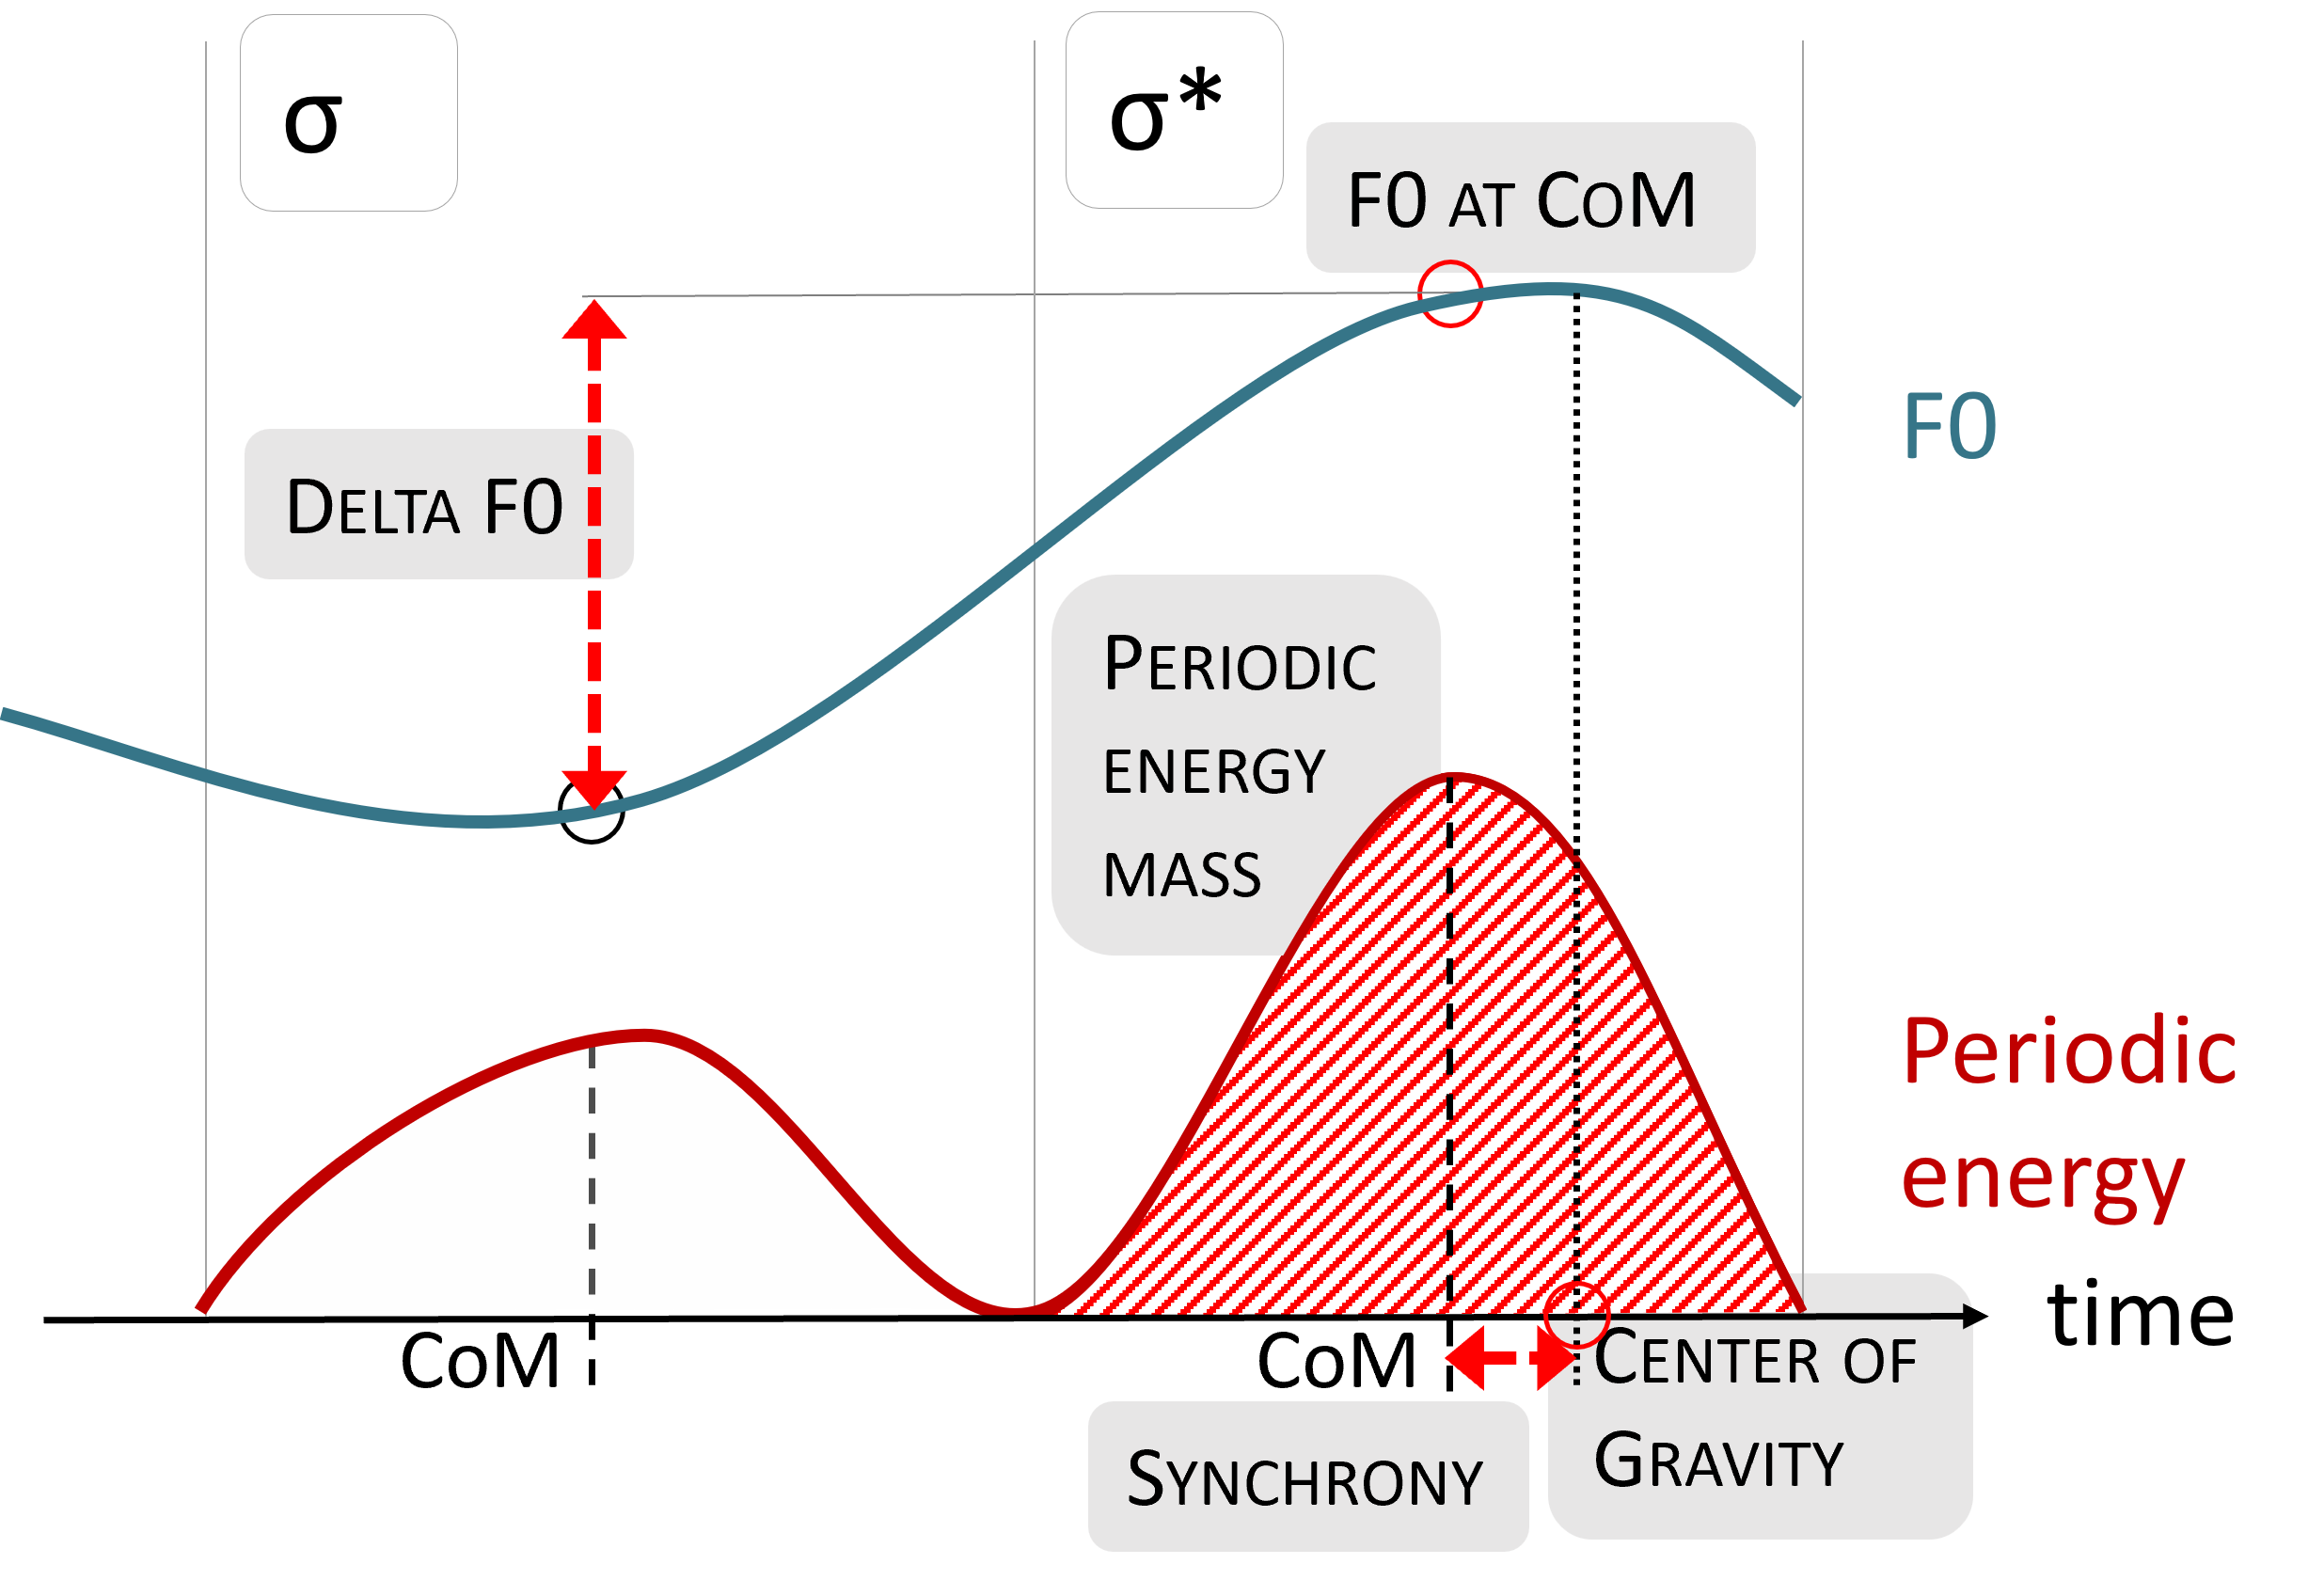
\includegraphics[scale = 0.5]{proper_schema}
	\caption{Schematic depiction of the ProPer measures, adapted from \citet{lorenzenParadigmaticSyntagmaticEffects2024}.}
	\label{fig:proper}
\end{figure}

\subsection{Statistical analysis} \label{sec: stats study1}

All analyses were conducted in R \citep{rcoreteamLanguageEnvironmentStatistical2022}, using the packages \pkg{tidyverse} \citep{wickhamWelcomeTidyverse2019}, \pkg{cowplot} \citep{wilkeCowplotStreamlinedPlot2020}, and \pkg{ggh4x} \citep{vandenbrandGgh4xHacksGgplot22024} for data wrangling and plotting, \pkg{brms} \citep{burknerBrmsPackageBayesian2017} as an interface to the Stan modeling language \citep{carpenterStanProbabilisticProgramming2017} for compiling regression models, and \pkg{cluster} \citep{maechlerClusterClusterAnalysis2022} for cluster analysis. The package \pkg{ggdendro} \citep{devriesGgdendroCreateDendrograms2024} was used to create a dendrogram. All data and scripts used to perform the analyses presented here are available from the accompanying OSF repository (\url{https://osf.io/m5xwe/}). 

We compiled separate Bayesian mixed-effects regression models for accent status, accent type, and each of the seven prosodic parameters. For the categorical parameters, we ran a binary logistic regression model using accent status as the dependent variable (levels: \textit{prenuclear}, \textit{nuclear}) and a cumulative regression model with accent type as the dependent variable. Here, we treated pitch accent type as an ordered factor according to the ranking established by \citet{baumannPerceptualProminencePitch2015}, namely, from most to least prominent: L+H* > L*+H > H* > H+!H* > H+L* > !H* > L*. The models for the continuous parameters contained the z-scored parameter as the dependent variable. Z-scoring was done to ensure the comparability of the different parameters despite the different units in which they were measured. Each model included information status (levels: \textit{new}, \textit{accessible}) and position (levels: \textit{Word1}, \textit{Word2}) as well as their interaction as predictors, random intercepts for speaker and word, and random slopes for the by-speaker effects of information status and position.\footnote{Note that the accent status model was run only on the subset of the data including Word1 and thus did not include position as a predictor since Word2 was always produced with a nuclear accent.} The random slopes capture the fact that speakers may differ in whether and to what degree they modulate certain parameters in order to encode information status, which makes them crucial to accounting for and analyzing inter-speaker variability.

Four sampling chains ran for 14,500 iterations with 12,000 warm-up iterations for a total of 10,000 posterior draws. We set weakly informative, normally distributed priors centered around zero with a standard deviation of one for the regression coefficients and used default priors provided by \pkg{brms} for the remaining model parameters. Model fits were assessed visually by inspecting the posterior predictive checks and by ensuring that the models yielded no Rhat values larger than one.

For each model, we report the regression coefficient $\beta$ and 90\% credible intervals (CrIs) under the posterior distributions as well as the posterior probability that $\beta$ is larger than zero: Pr($\beta$\textgreater{}0). While the interpretation of a Bayesian regression model allows for a gradient evaluation of the effects under investigation, it is useful to specify reliability criteria that allow for a binary decision, which facilitates comparisons to analyses conducted in the frequentist framework. We thus consider the effect of a contrast specified by the predictor variables ``reliable" if the 90\% credible interval (CrI) does not include 0 and the probability that $\beta$ is larger than zero is higher than 0.95 or lower than 0.05. 

For a systematic approach to investigating individual speaker strategies, we extracted the random slope estimates from the models with the continuous dependent variables and ran a hierarchical agglomerative cluster analysis on those estimates.\footnote{Note that we conduct this analysis only on the continuous variables, which were modeled via linear regression. The categorical variables were modeled via logistic and cumulative regression, so that the model estimates are on a different scale, namely log odds. Running the same cluster analysis on these differently scaled numbers would confound the results.} This analysis is modeled after \citet{baumannWhatMakesWord2018}, who conducted a similar analysis on the random slopes of their frequentist models. First, a distance matrix was computed, estimating the Euclidean distances between the random slope estimates. Second, a hierarchical cluster analysis was performed on this distance matrix using the Ward D.2 algorithm. The clustering algorithm operates bottom-up, i.e., initially, every speaker represents their own cluster and then the speakers with the smallest distances are grouped together iteratively until all speakers are merged together in one cluster. In order to determine the optimal number of clusters, we rely on the average silhouette width. Silhouette width is a measure of well-formedness of clusters, quantifying how similar members of the same cluster are to each other and how dissimilar members of different clusters are. Silhouette width values range from 0 to 1 with 0 indicating that there is no cluster structure in the data and 1 meaning that all data cluster perfectly into separate groups \citep{levshinaHowLinguisticsData2015}. A silhouette width above 0.25 can be interpreted as reasonable evidence for a cluster structure being present in the data \citep[88]{kaufmanFindingGroupsData1990}. 

\section{Results} \label{sec:Production 1 results}

\subsection{Overall results} \label{sec:Production 1 overall results}

This section considers the overall results averaged across all speakers to establish a baseline, which allows for comparisons regarding how and to what extent individuals differ from this group average. Figure \ref{fig:example_pitchtracks} shows two exemplary productions of the two target noun phrases in two different utterances produced by two different speakers to illustrate the general structure of the data.\footnote{These figures were created using the R package \pkg{praatpicture} \citep{puggaard-rodePraatpicturePraatPicture2024}.} In the utterance visualized in the top panel, the target words were produced with a typical hat pattern, a rising accent on Word1 and a falling accent on Word2, which is very frequent in our data. The utterance in the bottom panel represents a common alternative production with two subsequent rising accents on the target words. Target words were always produced with a pitch accent (prenuclear or nuclear), which was annotated on the Accent type tier. Due to the nature of the target sentences, phrase boundaries were very frequently produced after the first target word (in 58\% of cases), as, for example, in the top panel of Figure \ref{fig:example_pitchtracks} but rarely after Word2 (only 4\%).

\begin{figure}

%     \subfloat{
    {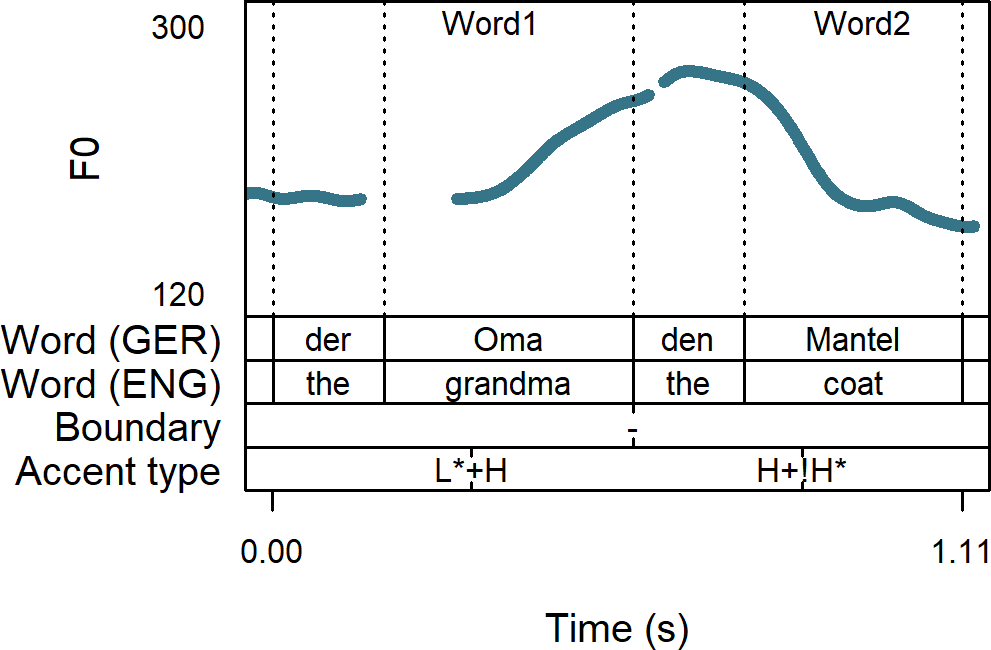
\includegraphics[width=.7\textwidth]{pitchtrack_s12oma_cropped.png} }
%     }

    \bigskip

%     \qquad
%     \subfloat{
    {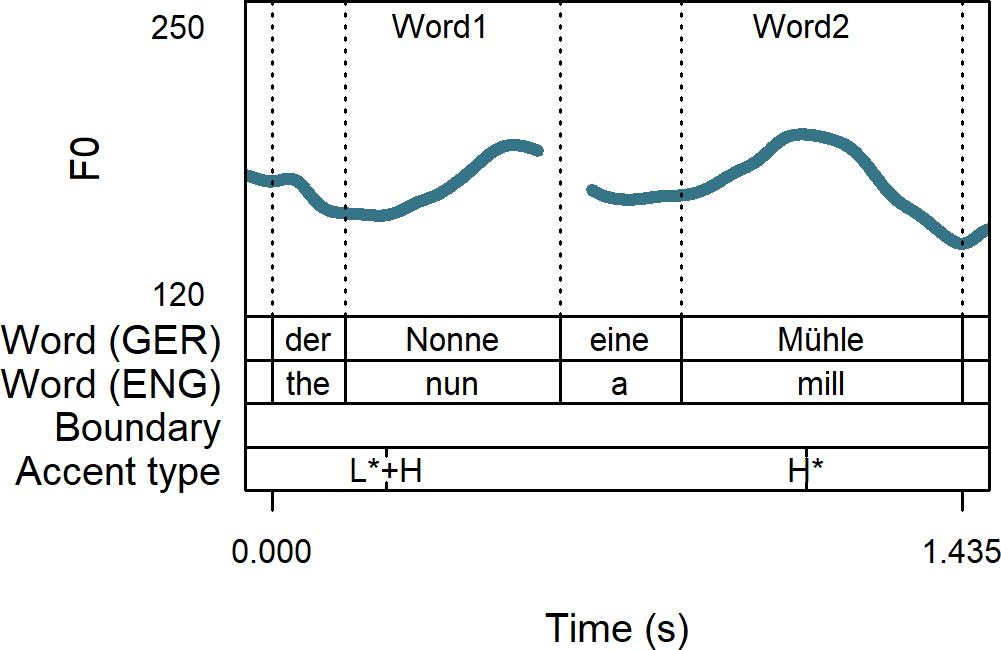
\includegraphics[width=.7\textwidth]{pitchtrack_s10nonne_cropped.png} }
%     }
    \caption{Examples of the F0 contour realized over the target words in two typical productions with DIMA boundary annotation and GToBI accent type.}
    \label{fig:example_pitchtracks}
\end{figure}

Since Word1 and Word2 were often produced differently, e.g., Word1 was always produced with a rising intonation, while Word2 often exhibits falling F0, we will consider the effects of information status on Word1 and Word2 separately for each prosodic parameter. In terms of metrical structure, Word2 was always produced with a nuclear accent, while Word1 either received a prenuclear or a nuclear accent depending on whether it was followed by a phrase boundary. Figure \ref{fig:s1_accent_statustype} (left) illustrates the distribution of accent status by word position and information status. It is evident that accent status in Word1 is probabilistically modulated by information status: New target words are more likely to be produced with a nuclear accent than accessible target words, i.e., the former tend to occupy metrically stronger, more prominent positions than the latter. According to the Bayesian regression model (see Table \ref{table:model_prosodic-discrete}), this effect is fairly strong, albeit not quite reliable following the criteria specified in Section \ref{sec: stats study1}.

\begin{figure}
		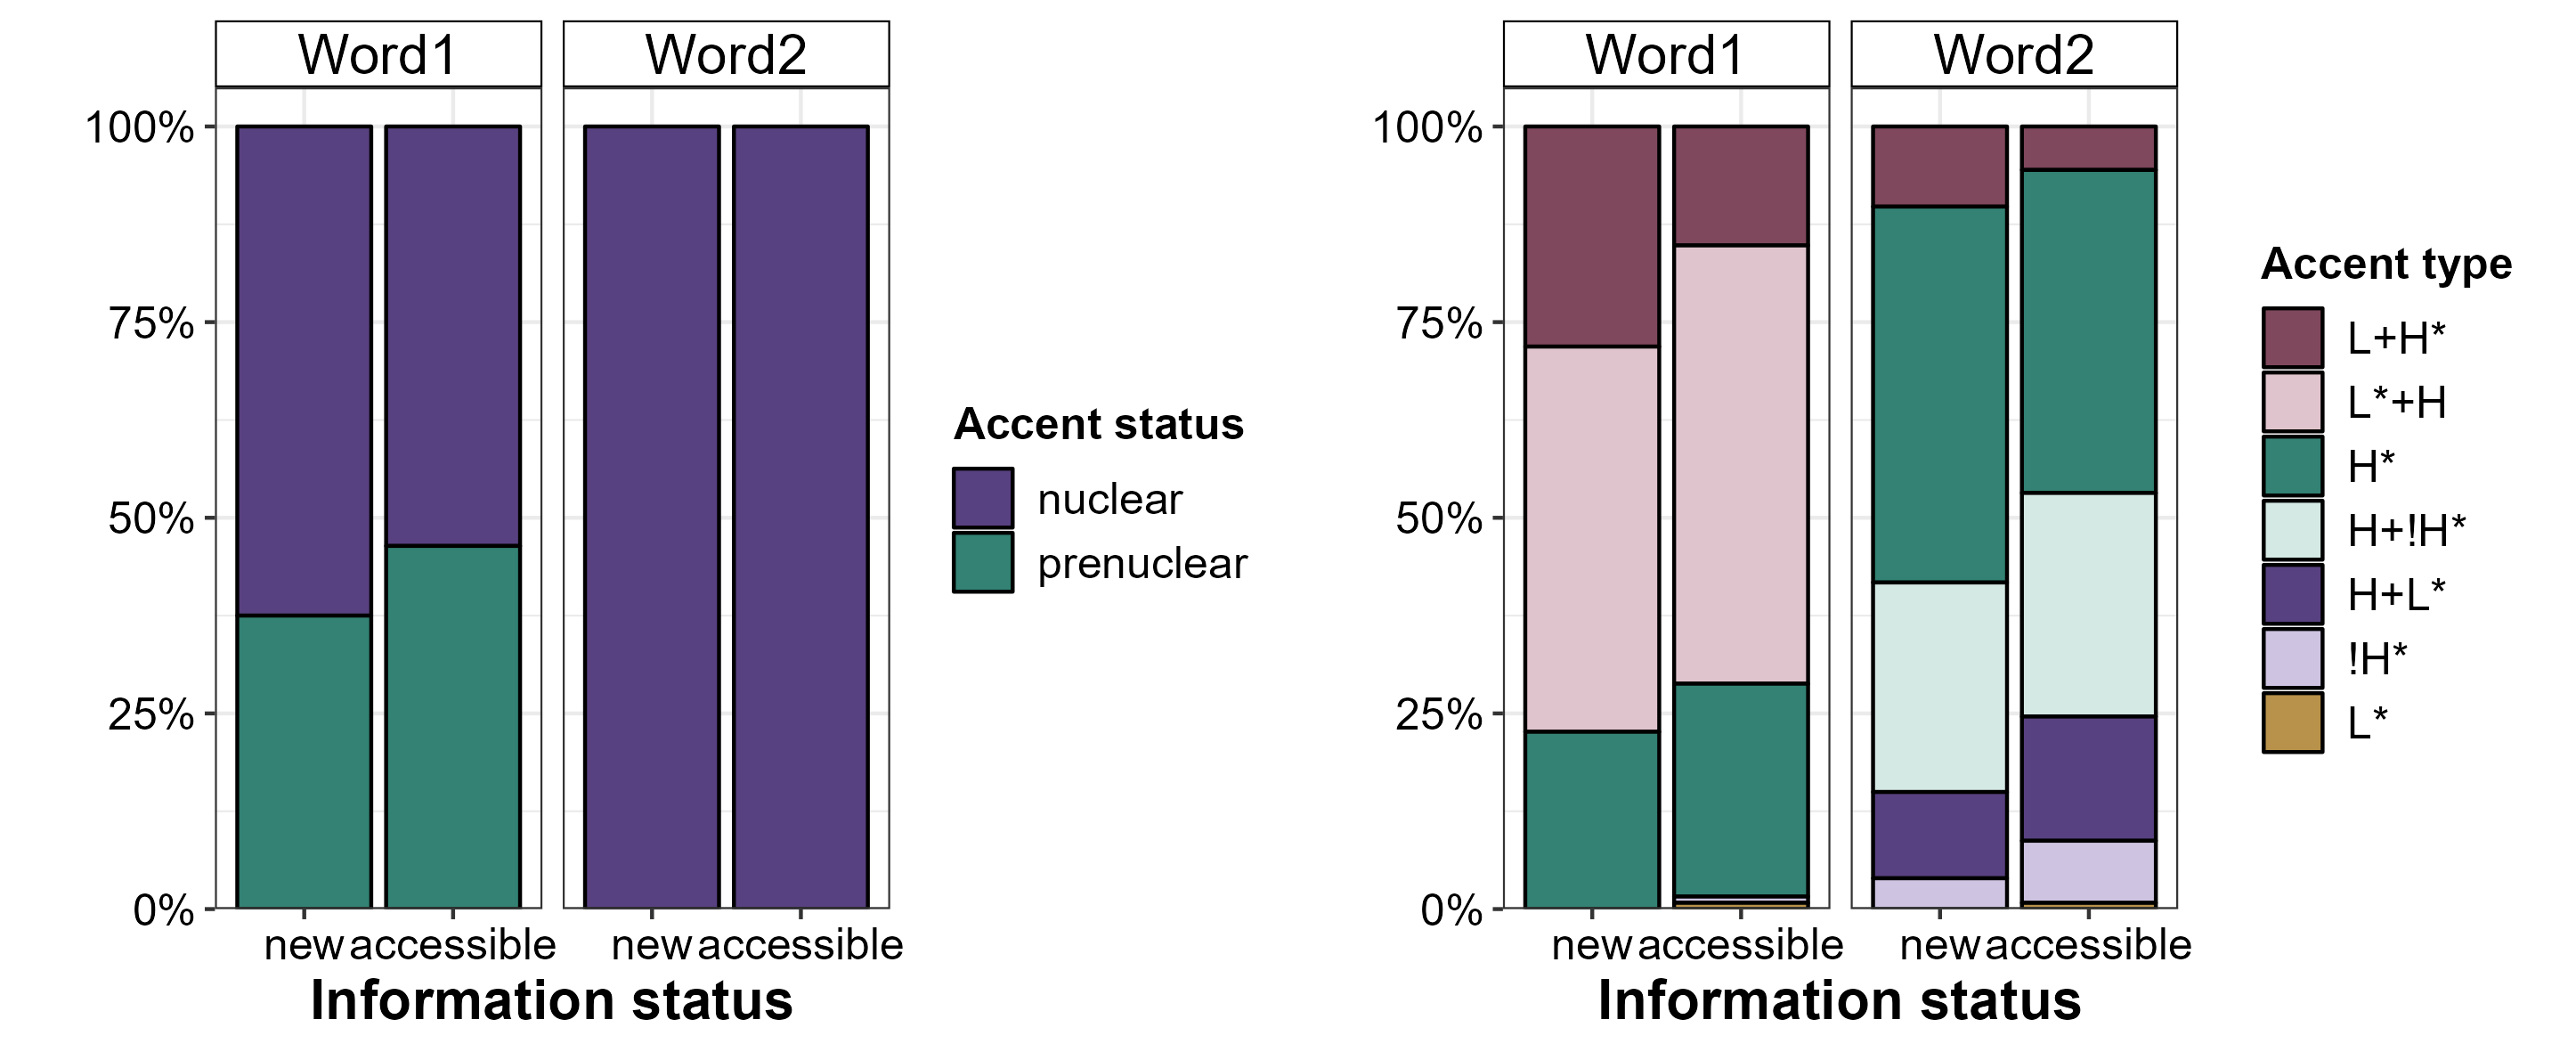
\includegraphics[scale = 0.5]{s1_accent_statustype}
	\caption{Barplots of the distributions of accent status and accent type by position and information status.}
	\label{fig:s1_accent_statustype}
\end{figure}

\begin{table}[]
\begin{tabular}{lrrr}
\lsptoprule
Variable    & $\beta$ & 90\% CrI  & Pr($\beta$\textgreater{}0) \\ \hline
Accent status (Word1)    & 0.12       & {[}0.00; 0.24{]}  & 0.95                          \\
Accent type (Word1)    & 0.61       & {[}0.21; 1.02{]}  & 0.99                          \\
Accent type (Word2)         & 0.66       & {[}0.23; 1.09{]} & 0.99                          \\
\lspbottomrule
\end{tabular}
\caption{Model parameters describing the effects of information status in the categorical prosodic parameters.}
\label{table:model_prosodic-discrete}
\end{table}

As for accent type, Figure \ref{fig:s1_accent_statustype} (right) illustrates the different accent type distributions produced on Word1 and Word2. Word1 was often produced with the high rising accents L*+H and L+H*, while falling accents, such as H+!H* and H+L*, occur only in Word2. Within each position, information status further modulates the likelihood of certain accent types occurring. Accent types in Figure \ref{fig:s1_accent_statustype} are ordered according to their inherent prominence following \citet{baumannPerceptualProminencePitch2015}. In both Word1 and Word2, new target words are produced with higher proportions of more prominent accent types, e.g., L+H* accents are more likely to be produced on new than on accessible target words, while accessible target words are more often produced with less prominent accent types, e.g., H* in Word 1 or H+L* and !H* in Word2. These differences are statistically reliable in both positions (see Table \ref{table:model_prosodic-discrete}).

Turning to the continuous phonetic parameters, Table \ref{table:model_parameters_Word1} summarizes the key model estimates for all continuous parameters for Word1. Generally, we expect higher values (associated with higher prominence) in new as compared to accessible referents for all continuous parameters (see also Section \ref{section: prominence form}), which is the case when the posterior estimate $\beta$ takes a positive value. In case of a negative $\beta$ estimate, the prosodic parameter in question takes on average higher values in accessible than in new referents. According to the reliability criteria specified in the previous section, Delta F0 is the only reliable cue to information status in Word1. More specifically, new referents are consistently produced with a higher Delta F0 than accessible referents. Higher F0 at CoM and longer word duration also appear to be relatively strong cues to newness. While synchrony displays a somewhat weaker tendency for higher values in the new referents, CoG and syllable duration do not appear to encode the information status contrast systematically. Finally, periodic energy mass exhibits an unexpected albeit weak tendency for higher values in accessible referents.

\begin{table}[]
\begin{tabular}{lrrr}
\lsptoprule
\multicolumn{4}{c}{Word1} \\ \hline
Variable    & $\beta$ & 90\% CrI  & Pr($\beta$\textgreater{}0) \\ \hline
F0 at CoM    & 0.12       & {[}0.00; 0.24{]}  & 0.95                          \\
Delta F0    & 0.30       & {[}0.15; 0.44{]}  & 1.00                          \\
Center of Gravity            & 0.03       & {[}-0.11; 0.16{]}  & 0.63                          \\
Synchrony            & 0.09       & {[}-0.04; 0.22{]}  & 0.88                          \\
Word duration            & 0.15       & {[}-0.01; 0.31{]}  & 0.94                          \\
Syllable duration & 0.05       & {[}-0.15; 0.24{]}  & 0.66                             \\
Periodic energy mass         & -0.10       & {[}-0.34; 0.14{]} & 0.25                          \\
\lspbottomrule
\end{tabular}
\caption{Model parameters describing the effects of information status in Word1.}
\label{table:model_parameters_Word1}
\end{table}

Regarding Word2 (see Table \ref{table:model_parameters_Word2}), again, Delta F0 emerges as the only reliable cue to information status, with new referents being produced with on average higher Delta F0 than accessible referents. There is also evidence that higher synchrony values are found in new referents. Unexpectedly, it appears that F0 at CoM is on average \textit{lower} in new than in accessible referents. A weaker tendency to be found is that word duration is longer in new than in accessible referents. CoG, syllable duration, and periodic energy mass again seem to play only a minor role in information status marking, similar to the findings for Word1.

\begin{table}[]
\begin{tabular}{lrrr}
\lsptoprule
\multicolumn{4}{c}{Word2} \\ \hline
Variable    & $\beta$ & 90\% CrI  & Pr($\beta$\textgreater{}0) \\ \hline
F0 at CoM    & -0.08       & {[}-0.20; 0.05{]}  & 0.15                          \\
Delta F0    & 0.43       & {[}0.29; 0.58{]}  & 1.00                          \\
Center of Gravity            & -0.06       & {[}-0.20; 0.08{]}  & 0.23                          \\
Synchrony            & 0.12       & {[}-0.01; 0.24{]}  & 0.93                          \\
Word duration            & 0.06       & {[}-0.04; 0.17{]}  & 0.85                          \\
Syllable duration & 0.05       & {[}-0.09; 0.17{]}  & 0.73                             \\
Periodic energy mass         & -0.03       & {[}-0.19; 0.14{]} & 0.40                          \\
\lspbottomrule
\end{tabular}
\caption{Model parameters describing the effects of information status in Word2.}
\label{table:model_parameters_Word2}
\end{table}

\subsection{Individual strategies}

After reporting on the averaged results across all speakers, this section explores how individual speakers might differ from or mirror this group behavior. As described in the previous section, both accent status (in Word1) and accent type are relatively strong cues to information status. However, this does not necessarily mean that all speakers make use of these phonological categories to encode information status or that they make use of them to the same extent. Figure \ref{fig:s1_accentstatus_byspeaker} displays the accent status distributions (only for Word1) for all speakers, showing considerable inter-individual variability. Four speakers, in fact, produce only nuclear accents (i.e., always produce a phrase boundary after Word1, third row in Figure \ref{fig:s1_accentstatus_byspeaker}) and one speaker (s24, fourth row) always realizes Word1 with a prenuclear accent. None of the speakers show a perfect one-to-one correspondence between nuclear accents on new referents on the one hand and prenuclear accents on accessible referents on the other, although speakers s2 and s18 (first row) come very close. Almost half of the speakers (n = 15) produce more nuclear accents in new referents, seven speakers make no difference between new and accessible and the remaining ten speakers show the reverse pattern, with more nuclear accents on accessible referents than on new ones.

\begin{figure}
		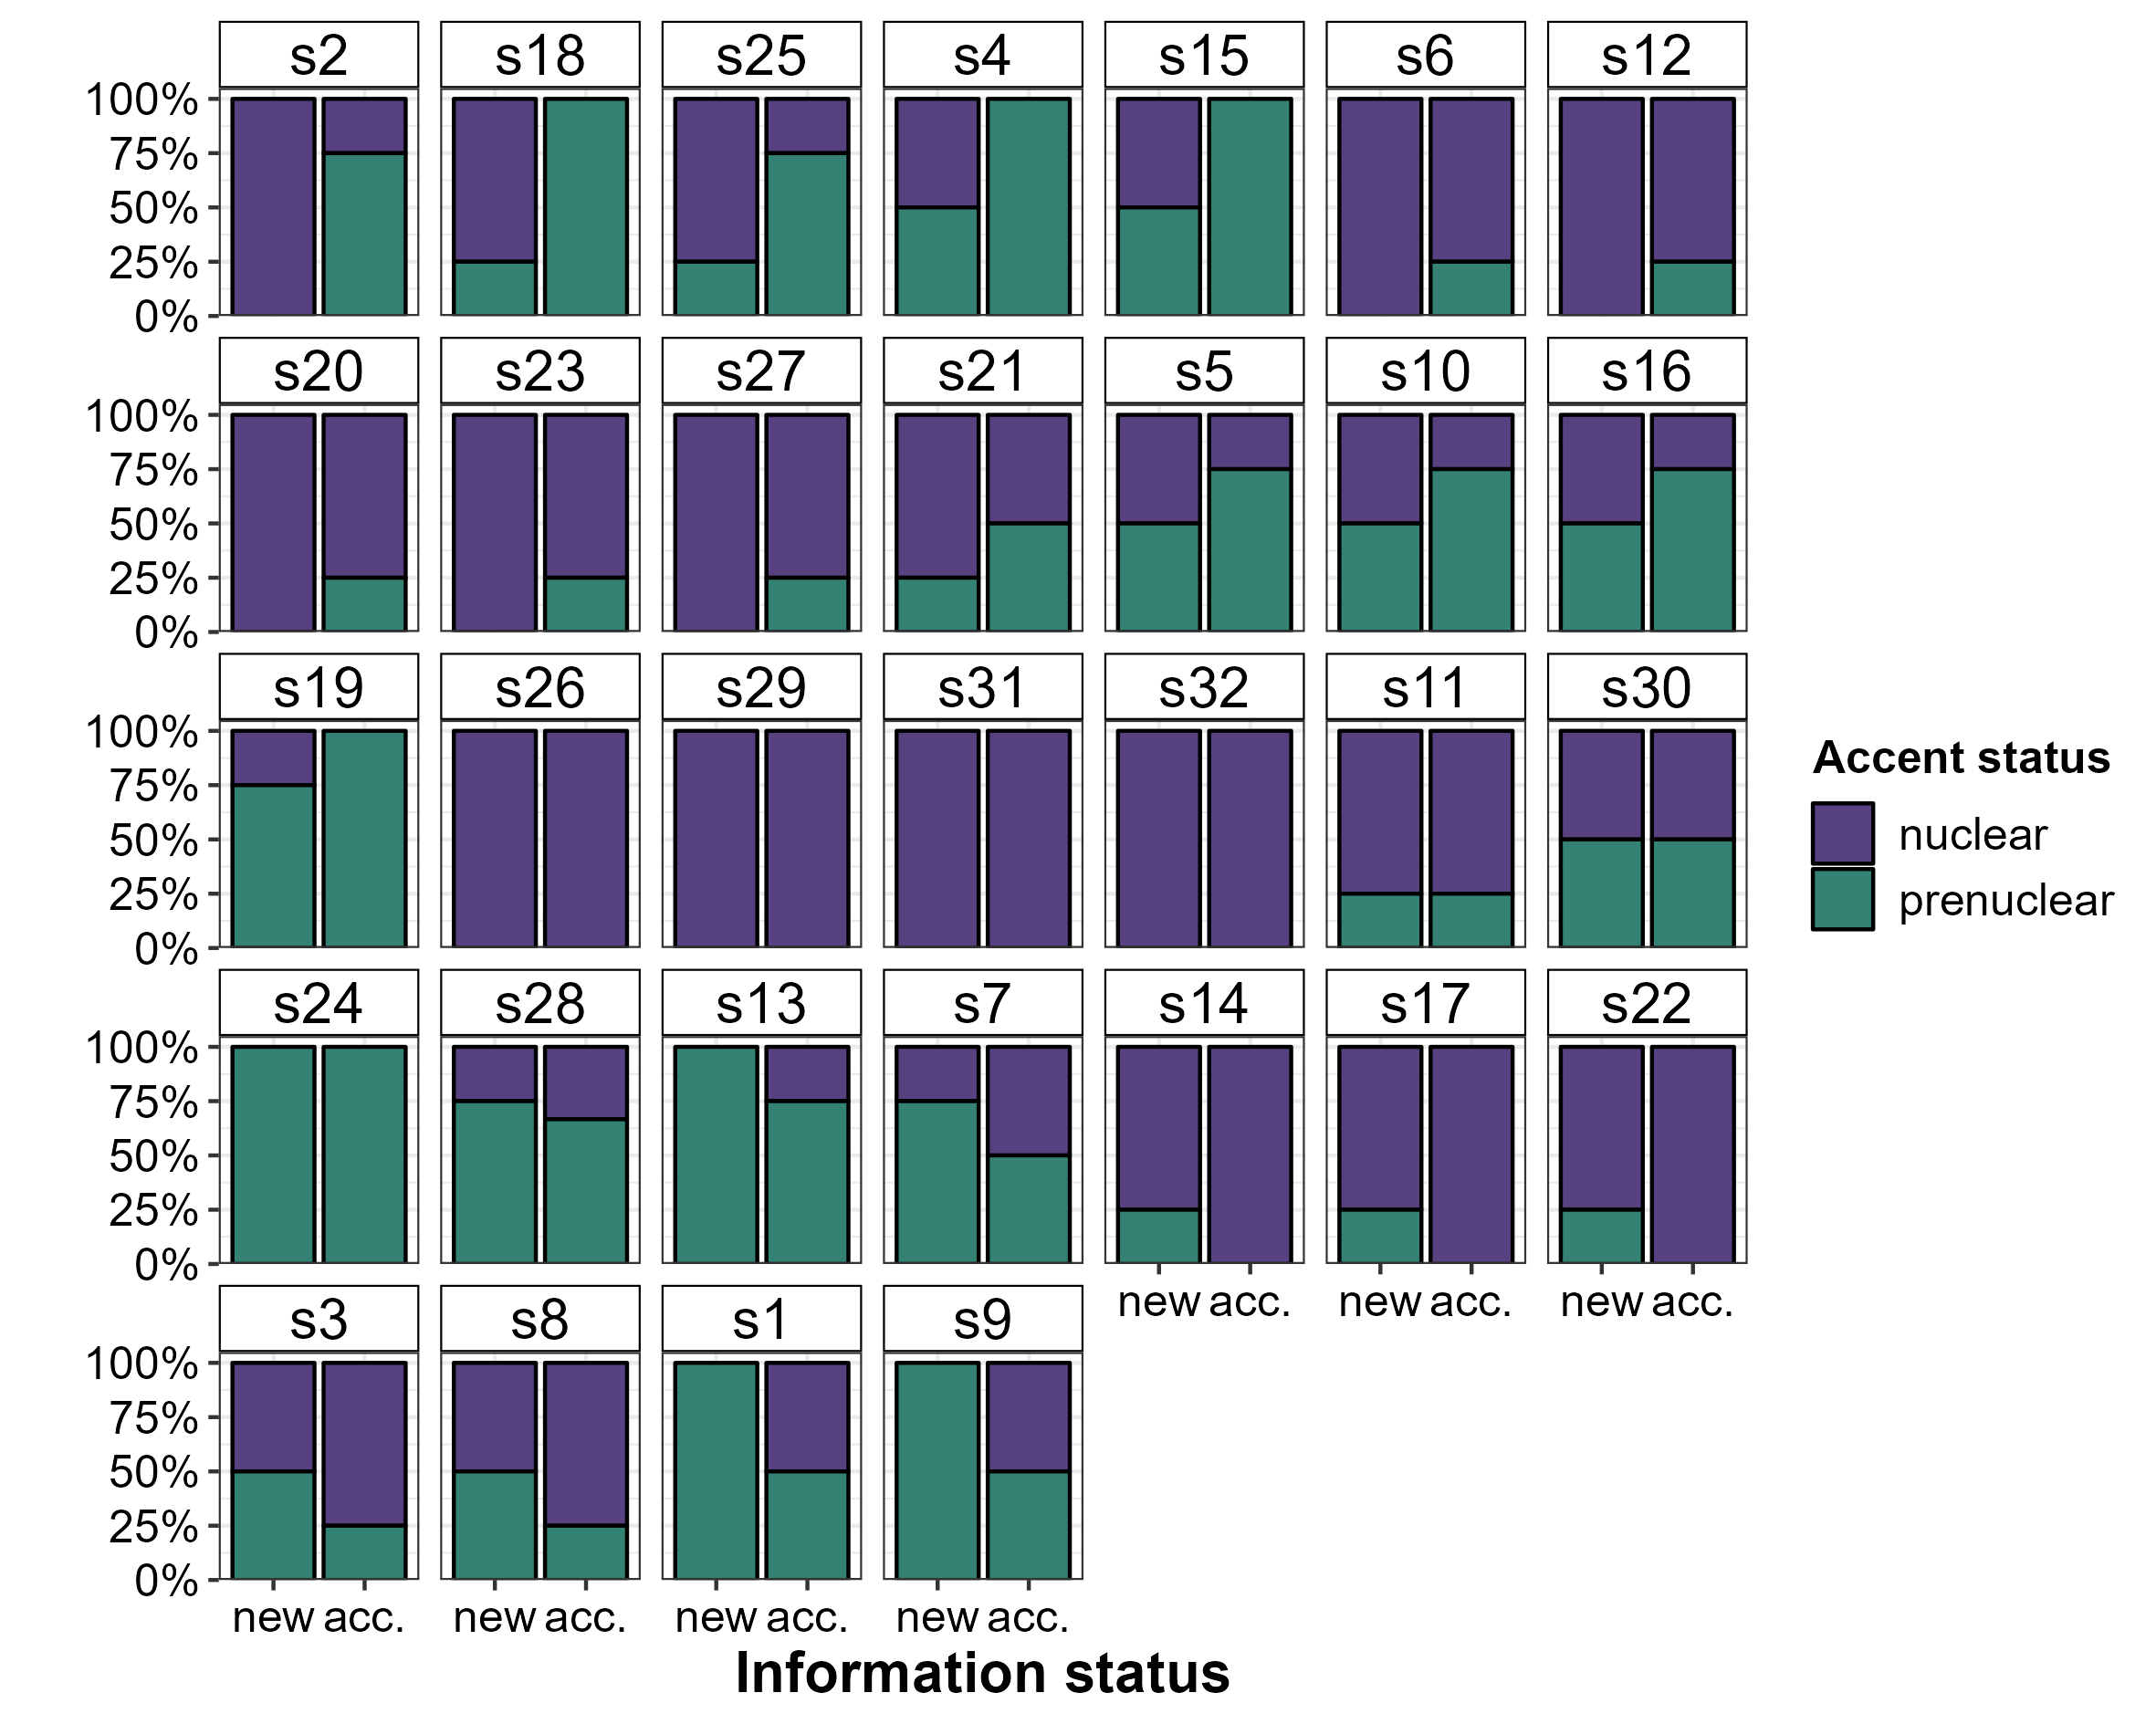
\includegraphics[scale = 0.6]{s1_accent_status_byspeaker}
	\caption{Barplots of accent status distributions on Word1 by information status per speaker.}
	\label{fig:s1_accentstatus_byspeaker}
\end{figure}

A comparable degree of variability emerges for pitch accent types. In Figure \ref{fig:s1_accenttype_byspeaker}, we consider eight exemplary speakers for reasons of space and ease of comprehensibility (plots for all speakers can be found in Appendix \ref{Appendix A}). Speakers vary in how many different accent types they produce, e.g., speaker s31 (top row, left) produces only two different accent types in both positions, while other speakers produce up to five different accent types across both positions. Generally, speakers are relatively consistent within their own productions, most using only one or two different accent types per position and information status condition. Crucially, there are differences in the use of accent type as a cue to information status. In Figure \ref{fig:s1_accenttype_byspeaker}, the two speakers in the top row show a tendency to produce new target words with more prominent accent types than accessible ones in both Word1 and Word2. This is in fact the pattern exhibited by the largest group of speakers (34\%). Interestingly, these two speakers (s31 and s26) both produce only nuclear accents on Word1 (see Figure \ref{fig:s1_accentstatus_byspeaker}), so that they potentially compensate for the absence of accent status as a cue to information status by producing accent type differences instead. The two speakers in the second row of Figure \ref{fig:s1_accenttype_byspeaker} produce more prominent accent types on new target words only in Word1, while there is no difference between new and accessible in Word2, which is a pattern repeated by 16\% of speakers in our data. The reverse strategy is embodied by the speakers in the third row (and in 28\% of our speakers), who produce more prominent accent types for new referents only in Word2. Finally, there are also speakers (22\% in our data), such as those in the bottom row of Figure \ref{fig:s1_accenttype_byspeaker}, who produce more prominent accent types on accessible target words as compared to new ones. Here, speaker s32 also produces only nuclear accents on Word1, so that neither categorical prosodic parameter serves as a cue to information status for this speaker. However, speakers failing to make categorical distinctions between new and accessible target words could still make use of more subtle phonetic cues to encode information status. 

\begin{figure}
		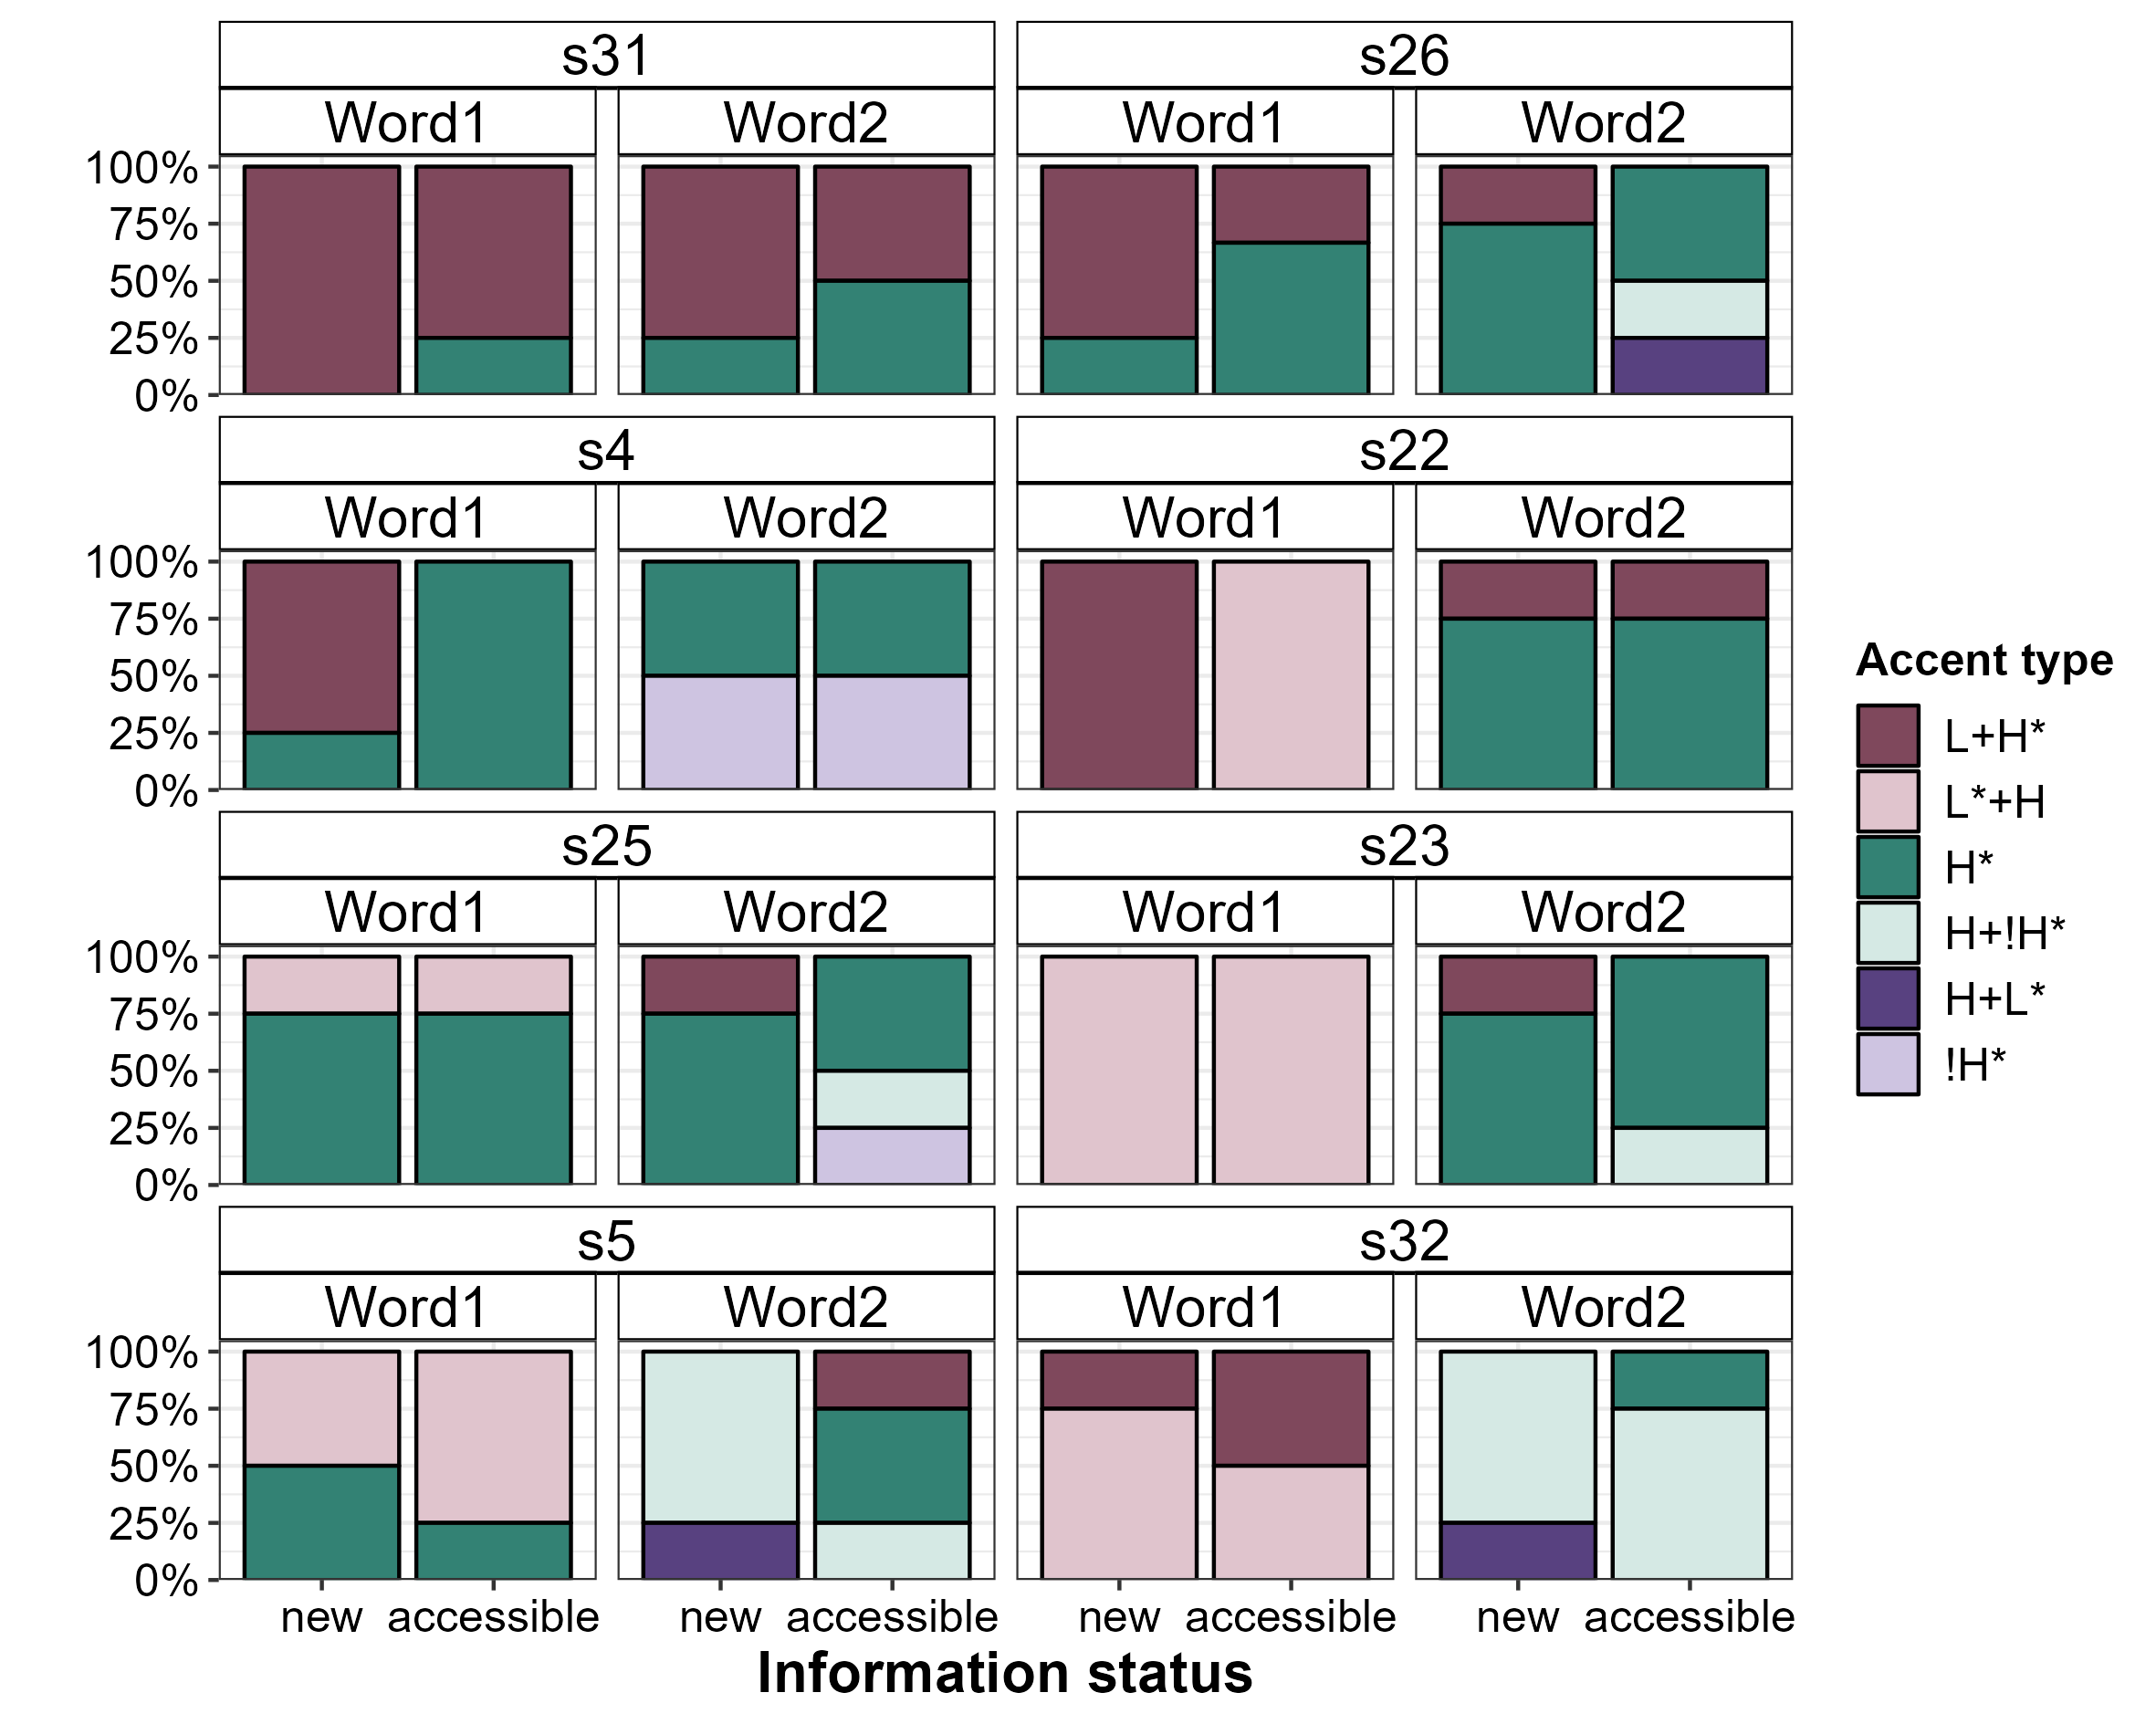
\includegraphics[scale = 0.6]{s1_accent_type_byspeaker}
	\caption{Barplots of accent type distributions by position and information status for eight exemplary speakers.}
	\label{fig:s1_accenttype_byspeaker}
\end{figure}

In Section \ref{sec:Production 1 overall results}, Delta F0 was the most reliable continuous prosodic cue to information status, with higher Delta F0 indicating newness and lower Delta F0 accessibility. However, this does not necessarily mean that every single speaker uses Delta F0 in this way. Word duration constitutes another relatively strong and consistent cue to information status across both word positions, which is nevertheless slightly less reliable than Delta F0. To illustrate how diverse speaker behavior can be beyond group averages, Figure \ref{fig:speaker_examples} depicts the distributions of z-scored Delta F0 and word duration values separated by information status for four exemplary speakers. Speaker s22 (Figure \ref{fig:speaker_examples}, top row) produces on average higher Delta F0 in new target words, however, the distributions of word duration for new and accessible target words are highly overlapping and the difference between the means is very small, indicating that this speaker makes use of Delta F0 but not duration to encode information status. For speaker s10 (Figure \ref{fig:speaker_examples}, second row), although there is quite a bit of overlap for the distributions of Delta F0 and word duration, both exhibit on average higher values in the new condition, so that both serve as a cue to newness for this speaker. By contrast, speaker s1 (Figure \ref{fig:speaker_examples}, third row) seems to use longer word duration for new as compared to accessible target words, but (if anything) slightly lower Delta F0. Finally, speaker s14 (Figure \ref{fig:speaker_examples}, bottom row) displays neither an effect of information status on Delta F0 nor on word duration, with both cue distributions largely overlapping. To summarize, by looking at four different speakers' use of two parameters, we find four different strategies, indicating that there may be as many different individual strategies as cue combinations.

\begin{figure}
		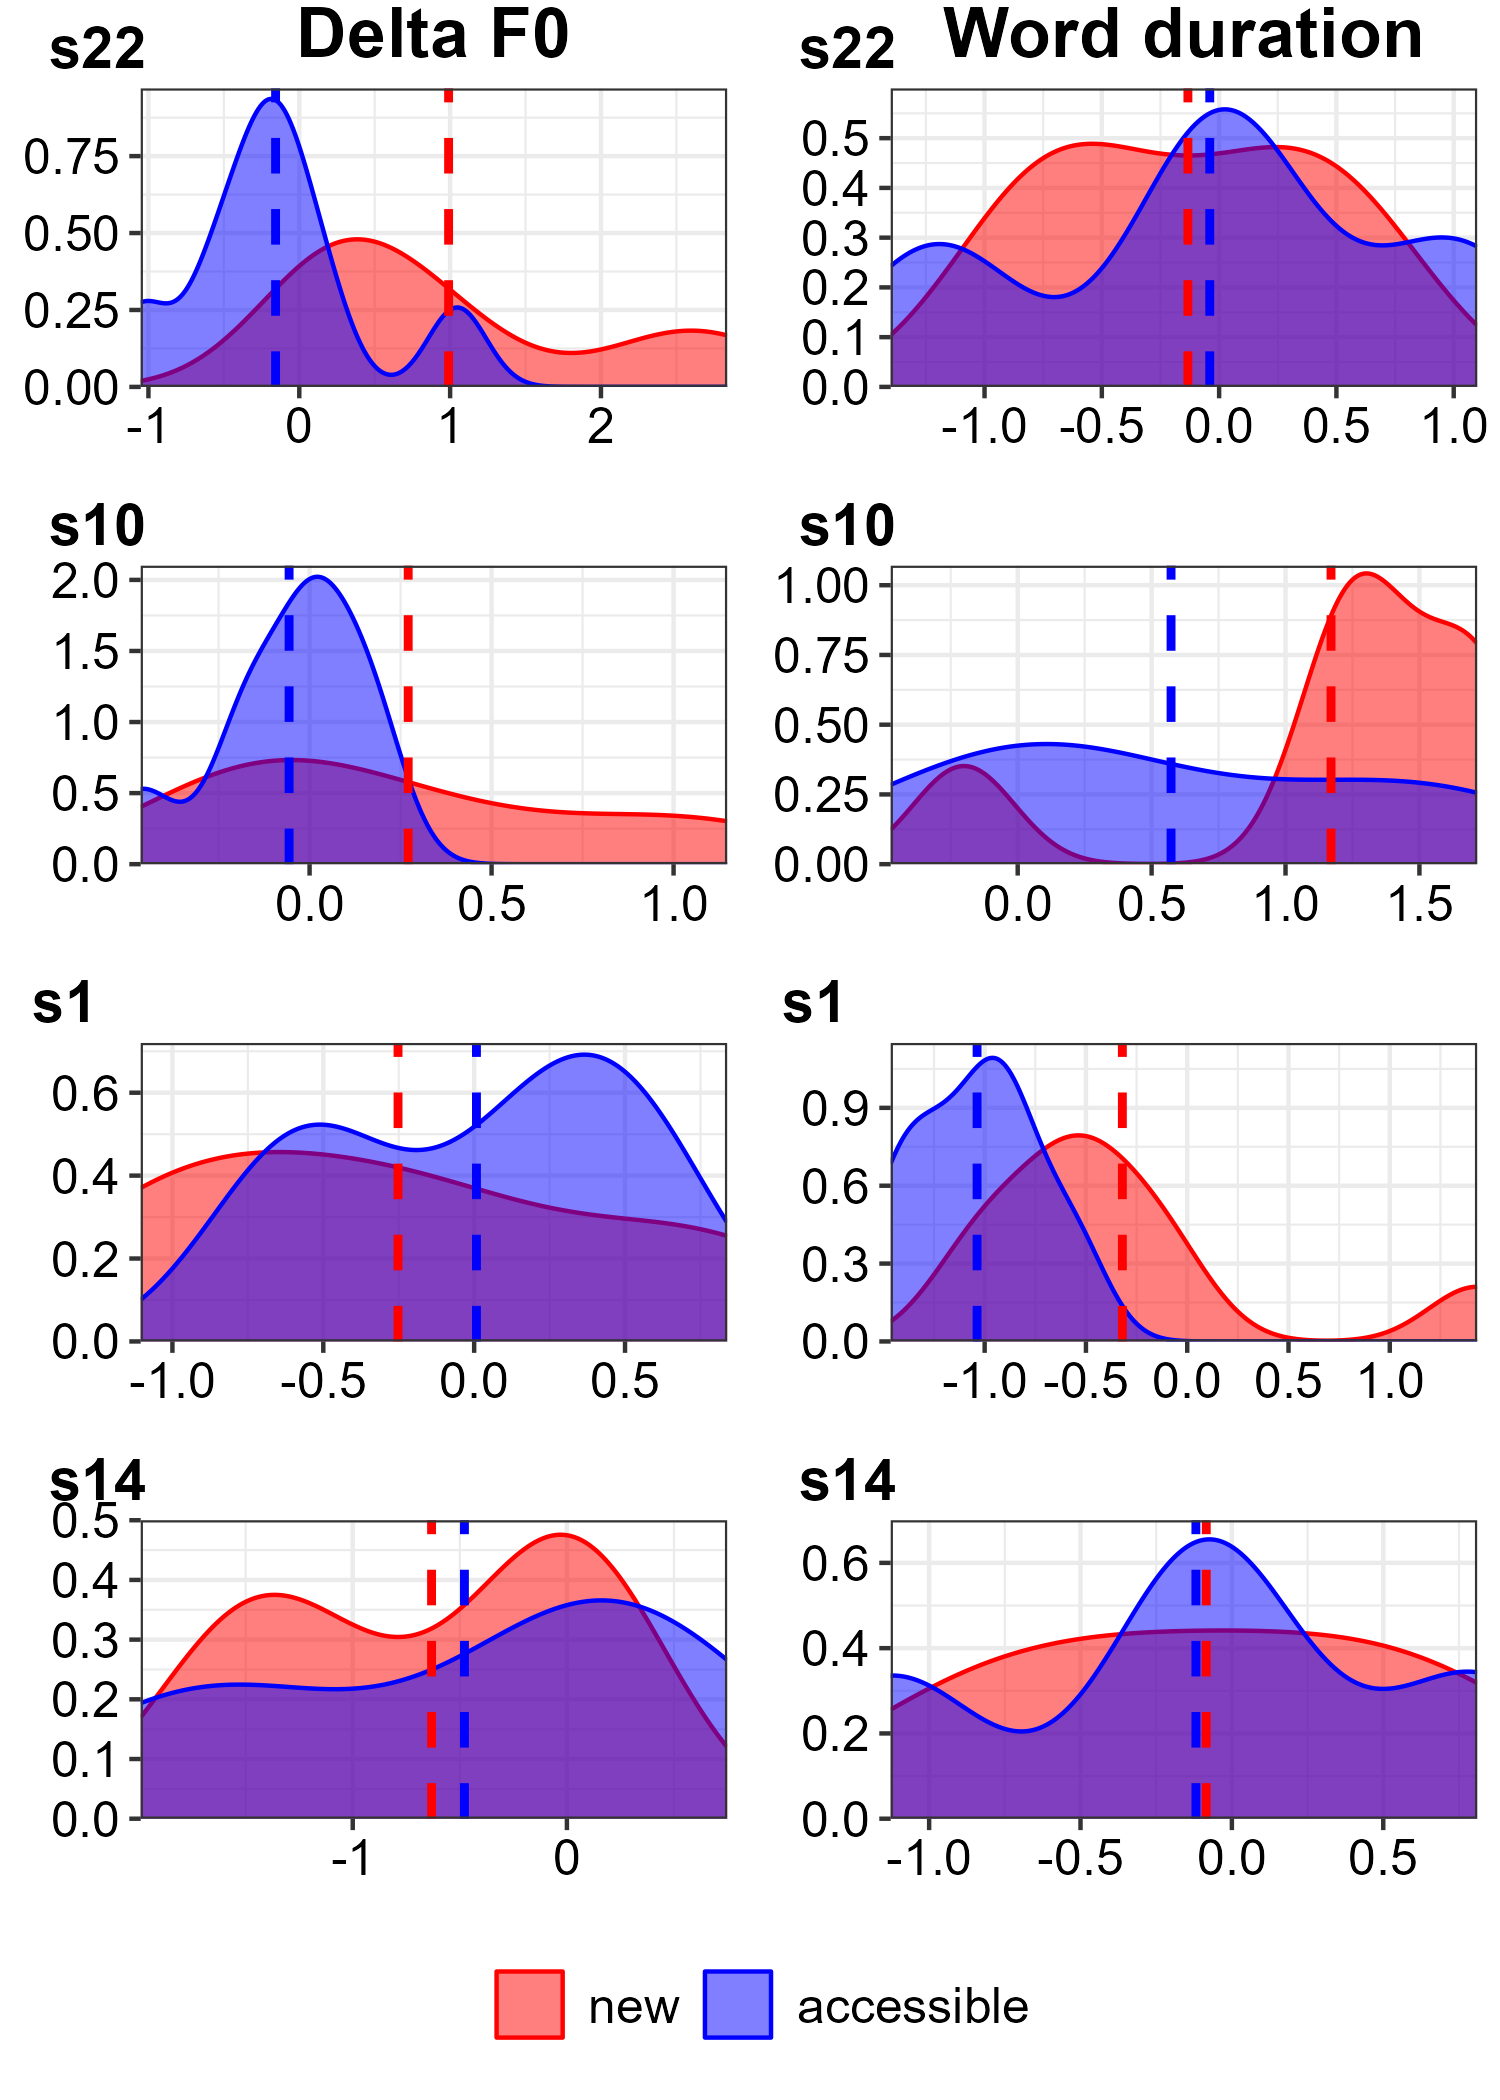
\includegraphics[scale = 0.6]{speaker_examples}
	\caption{Plots showing distributions and means (dashed lines) of z-scored Delta F0 (left panels) and word duration (right panels) by information status for four exemplary speakers.}
	\label{fig:speaker_examples}
\end{figure}

For a more complete picture of individual speakers' usage of all seven prosodic parameters investigated here, Table \ref{table:zscore_diffs} summarizes the differences between new and accessible target words in the z-scored parameters per speaker. Here, darker shading indicates larger positive differences, i.e., the parameters serve as stronger cues to information status in the expected direction with higher values for new than for accessible target words. Focusing first on the columns, it is apparent that higher Delta F0 is used by most speakers to mark newness (25 out of 32), which reflects the result of Delta F0 being the strongest cue to information status overall. Nevertheless, some speakers do not seem to make use of Delta F0 in this way, instead relying on other parameters. For example, speaker s1 marks newness only by longer word and syllable duration, whereas all other parameters are unexpectedly higher in accessible than in new words. Speaker s5 does not appear to modulate any of the parameters in the expected direction, which is evident from the mostly negative differences in the respective row. In contrast, speaker s19 encodes information status maximally redundantly, making use of all seven continuous prosodic parameters. These latter two speakers represent the most extreme cases of information status marking, with a variety of different strategies existing on the continuum between these two points.

\begin{table}[]
\begin{tabular}{llllllll}
\lsptoprule
             & \begin{tabular}[c]{@{}l@{}}F0 at \\ CoM\end{tabular} & \begin{tabular}[c]{@{}l@{}}Delta \\ F0\end{tabular} & \begin{tabular}[c]{@{}l@{}}Center\\ of \\ Gravity\end{tabular} & Synchrony           & \begin{tabular}[c]{@{}l@{}}Word\\ duration\end{tabular} & \begin{tabular}[c]{@{}l@{}}Syllable\\ duration\end{tabular} & \begin{tabular}[c]{@{}l@{}}Periodic \\ energy\\ mass\end{tabular} \\ \hline
s1  & -0.29                                                         & -0.26                                                        & -0.47                                                                   & -0.21                        & \cellcolor[HTML]{9B9B9B}0.72                                     & \cellcolor[HTML]{9B9B9B}0.68                                         & -0.08                                                                      \\
s2  & -0.17                                                         & \cellcolor[HTML]{C0C0C0}0.42                                 & \cellcolor[HTML]{C0C0C0}0.17                                            & \cellcolor[HTML]{C0C0C0}0.43 & \cellcolor[HTML]{EFEFEF}0.08                                     & \cellcolor[HTML]{C0C0C0}0.34                                         & \cellcolor[HTML]{9B9B9B}0.97                                               \\
s3  & \cellcolor[HTML]{C0C0C0}0.49                                  & \cellcolor[HTML]{C0C0C0}0.27                                 & \cellcolor[HTML]{C0C0C0}0.20                                            & -0.08                        & \cellcolor[HTML]{EFEFEF}0.03                                     & -0.28                                                                & -1.16                                                                      \\
s4  & -0.09                                                         & \cellcolor[HTML]{C0C0C0}0.10                                 & -0.15                                                                   & \cellcolor[HTML]{EFEFEF}0.07 & 0.00                                                             & -0.10                                                                & \cellcolor[HTML]{C0C0C0}0.54                                               \\
s5  & -0.20                                                         & -0.23                                                        & -1.09                                                                   & -0.67                        & \cellcolor[HTML]{EFEFEF}0.05                                     & -0.33                                                                & -0.43                                                                      \\
s6  & \cellcolor[HTML]{EFEFEF}0.03                                  & \cellcolor[HTML]{9B9B9B}0.85                                 & -0.03                                                                   & \cellcolor[HTML]{C0C0C0}0.32 & -0.64                                                            & -0.51                                                                & NA                                                                         \\
s7  & -0.05                                                         & \cellcolor[HTML]{C0C0C0}0.28                                 & \cellcolor[HTML]{C0C0C0}0.10                                            & \cellcolor[HTML]{C0C0C0}0.32 & -0.13                                                            & -0.15                                                                & -0.41                                                                      \\
s8  & \cellcolor[HTML]{C0C0C0}0.37                                  & \cellcolor[HTML]{C0C0C0}0.13                                 & -0.13                                                                   & \cellcolor[HTML]{EFEFEF}0.05 & \cellcolor[HTML]{C0C0C0}0.58                                     & \cellcolor[HTML]{C0C0C0}0.44                                         & \cellcolor[HTML]{C0C0C0}0.35                                               \\
s9  & \cellcolor[HTML]{C0C0C0}0.39                                  & \cellcolor[HTML]{C0C0C0}0.53                                 & \cellcolor[HTML]{C0C0C0}0.27                                            & \cellcolor[HTML]{C0C0C0}0.22 & -0.06                                                            & -0.23                                                                & -0.04                                                                      \\
s10 & -0.14                                                         & \cellcolor[HTML]{C0C0C0}0.33                                 & -0.62                                                                   & -0.08                        & \cellcolor[HTML]{C0C0C0}0.60                                     & \cellcolor[HTML]{C0C0C0}0.49                                         & \cellcolor[HTML]{C0C0C0}0.53                                               \\
s11 & -0.42                                                         & \cellcolor[HTML]{C0C0C0}0.31                                 & \cellcolor[HTML]{9B9B9B}0.64                                            & \cellcolor[HTML]{C0C0C0}0.36 & \cellcolor[HTML]{EFEFEF}0.06                                     & \cellcolor[HTML]{C0C0C0}0.32                                         & \cellcolor[HTML]{9B9B9B}0.93                                               \\
s12 & \cellcolor[HTML]{EFEFEF}0.05                                  & \cellcolor[HTML]{EFEFEF}0.06                                 & \cellcolor[HTML]{EFEFEF}0.01                                            & \cellcolor[HTML]{C0C0C0}0.27 & -0.44                                                            & -0.50                                                                & -0.58                                                                      \\
s13 & \cellcolor[HTML]{EFEFEF}0.09                                  & \cellcolor[HTML]{C0C0C0}0.27                                 & \cellcolor[HTML]{9B9B9B}0.64                                            & \cellcolor[HTML]{EFEFEF}0.04 & \cellcolor[HTML]{EFEFEF}0.08                                     & \cellcolor[HTML]{C0C0C0}0.33                                         & -0.66                                                                      \\
s14 & -0.41                                                         & -0.15                                                        & -0.17                                                                   & \cellcolor[HTML]{C0C0C0}0.20 & \cellcolor[HTML]{EFEFEF}0.03                                     & -0.59                                                                & -0.57                                                                      \\
s15 & \cellcolor[HTML]{C0C0C0}0.54                                  & \cellcolor[HTML]{9B9B9B}0.96                                 & -0.06                                                                   & \cellcolor[HTML]{C0C0C0}0.26 & \cellcolor[HTML]{C0C0C0}0.15                                     & \cellcolor[HTML]{C0C0C0}0.21                                         & -1.16                                                                      \\
s16 & -0.54                                                         & -0.14                                                        & \cellcolor[HTML]{C0C0C0}0.21                                            & \cellcolor[HTML]{C0C0C0}0.29 & \cellcolor[HTML]{C0C0C0}0.21                                     & \cellcolor[HTML]{C0C0C0}0.52                                         & -0.60                                                                      \\
s17 & -0.26                                                         & \cellcolor[HTML]{9B9B9B}0.82                                 & -0.10                                                                   & \cellcolor[HTML]{C0C0C0}0.37 & -0.12                                                            & -0.38                                                                & \cellcolor[HTML]{C0C0C0}0.19                                               \\
s18 & -0.12                                                         & \cellcolor[HTML]{C0C0C0}0.28                                 & -0.01                                                                   & -0.29                        & \cellcolor[HTML]{C0C0C0}0.41                                     & \cellcolor[HTML]{9B9B9B}0.71                                         & \cellcolor[HTML]{C0C0C0}0.56                                               \\
s19 & \cellcolor[HTML]{C0C0C0}0.49                                  & \cellcolor[HTML]{9B9B9B}0.80                                 & \cellcolor[HTML]{9B9B9B}1.06                                            & \cellcolor[HTML]{9B9B9B}0.94 & \cellcolor[HTML]{C0C0C0}0.22                                     & \cellcolor[HTML]{C0C0C0}0.34                                         & \cellcolor[HTML]{C0C0C0}0.48                                               \\
s20 & \cellcolor[HTML]{9B9B9B}0.63                                  & \cellcolor[HTML]{9B9B9B}0.83                                 & -0.41                                                                   & \cellcolor[HTML]{C0C0C0}0.29 & -0.85                                                            & -1.05                                                                & \cellcolor[HTML]{C0C0C0}0.12                                               \\
s21 & -0.01                                                         & \cellcolor[HTML]{C0C0C0}0.13                                 & \cellcolor[HTML]{C0C0C0}0.35                                            & -0.50                        & \cellcolor[HTML]{C0C0C0}0.14                                     & \cellcolor[HTML]{9B9B9B}0.68                                         & -0.29                                                                      \\
s22 & \cellcolor[HTML]{9B9B9B}1.35                                  & \cellcolor[HTML]{9B9B9B}1.15                                 & -1.09                                                                   & -0.03                        & -0.09                                                            & -0.74                                                                & -0.50                                                                      \\
s23 & \cellcolor[HTML]{EFEFEF}0.02                                  & \cellcolor[HTML]{9B9B9B}0.94                                 & \cellcolor[HTML]{9B9B9B}0.73                                            & \cellcolor[HTML]{C0C0C0}0.41 & NA                                                               & NA                                                                   & NA                                                                         \\
s24 & \cellcolor[HTML]{EFEFEF}0.06                                  & \cellcolor[HTML]{C0C0C0}0.35                                 & -0.50                                                                   & \cellcolor[HTML]{C0C0C0}0.23 & -0.05                                                            & \cellcolor[HTML]{EFEFEF}0.01                                         & \cellcolor[HTML]{C0C0C0}0.40                                               \\
s25 & \cellcolor[HTML]{C0C0C0}0.12                                  & \cellcolor[HTML]{C0C0C0}0.45                                 & -0.39                                                                   & -0.09                        & \cellcolor[HTML]{C0C0C0}0.12                                     & -0.08                                                                & -0.44                                                                      \\
s26 & \cellcolor[HTML]{C0C0C0}0.14                                  & \cellcolor[HTML]{9B9B9B}0.88                                 & -0.04                                                                   & \cellcolor[HTML]{9B9B9B}0.63 & \cellcolor[HTML]{9B9B9B}0.77                                     & \cellcolor[HTML]{9B9B9B}0.83                                         & \cellcolor[HTML]{9B9B9B}1.04                                               \\
s27 & -0.16                                                         & \cellcolor[HTML]{C0C0C0}0.25                                 & \cellcolor[HTML]{EFEFEF}0.09                                            & -0.43                        & -0.08                                                            & \cellcolor[HTML]{C0C0C0}0.58                                         & -0.21                                                                      \\
s28 & -0.54                                                         & -0.08                                                        & -0.33                                                                   & \cellcolor[HTML]{C0C0C0}0.29 & -0.14                                                            & -0.33                                                                & \cellcolor[HTML]{9B9B9B}0.64                                               \\
s29 & -0.16                                                         & \cellcolor[HTML]{C0C0C0}0.17                                 & -0.36                                                                   & \cellcolor[HTML]{C0C0C0}0.10 & \cellcolor[HTML]{C0C0C0}0.37                                     & \cellcolor[HTML]{C0C0C0}0.24                                         & -0.30                                                                      \\
s30 & \cellcolor[HTML]{EFEFEF}0.09                                  & \cellcolor[HTML]{C0C0C0}0.39                                 & \cellcolor[HTML]{9B9B9B}0.80                                            & -0.01                        & -0.11                                                            & \cellcolor[HTML]{EFEFEF}0.09                                         & \cellcolor[HTML]{C0C0C0}0.14                                               \\
s31 & -0.02                                                         & \cellcolor[HTML]{9B9B9B}0.74                                 & -0.03                                                                   & \cellcolor[HTML]{C0C0C0}0.27 & -0.02                                                            & -0.32                                                                & -0.30                                                                      \\
s32 & -0.62                                                         & -0.18                                                        & -0.18                                                                   & -0.31                        & \cellcolor[HTML]{C0C0C0}0.30                                     & \cellcolor[HTML]{EFEFEF}0.02                                         & \cellcolor[HTML]{C0C0C0}0.10                                               \\
\lspbottomrule
\end{tabular}
\caption{Differences between new and accessible target words for z-scored prosodic parameters per speaker. Darker shading indicates larger positive differences.}
\label{table:zscore_diffs}
\end{table}

To complement the exploratory, descriptive approach to individual strategies presented above with a more systematic analysis, we conducted a cluster analysis to determine whether any groups of speakers can be established who, within their group, produce information status contrasts in a similar way but differ from other groups. Specifically, the random slope estimates from the Bayesian models presented in the previous section will be exploited to investigate whether any prominence cues are correlated across speakers, i.e., whether speakers group by which parameters they use in combination and how similar or dissimilar they are from each other. To ensure the comparability of the random slope estimates, we only include the models on the continuous z-scored variables in this analysis. The resulting clusters are illustrated by the dendrogram in Figure \ref{fig:s1_clusters} (left), where the purple box (top) includes the speakers assigned to Cluster 1 and the green box (bottom) the speakers assigned to Cluster 2. The dendrogram illustrates the agglomerative clustering process during which each speaker first represents their own cluster and then iteratively merges with similar speakers until finally all speakers are merged. According to the average silhouette width (0.28), a separation into two clusters is most appropriate for the data. Cluster 1 consists of ten speakers, Cluster 2 of 21 speakers.\footnote{Note that one speaker was not included in the cluster analysis because we excluded their periodic energy mass measures due to clipped audio recordings and thus no random slopes for this parameter were estimated for this speaker.}

\begin{figure}
		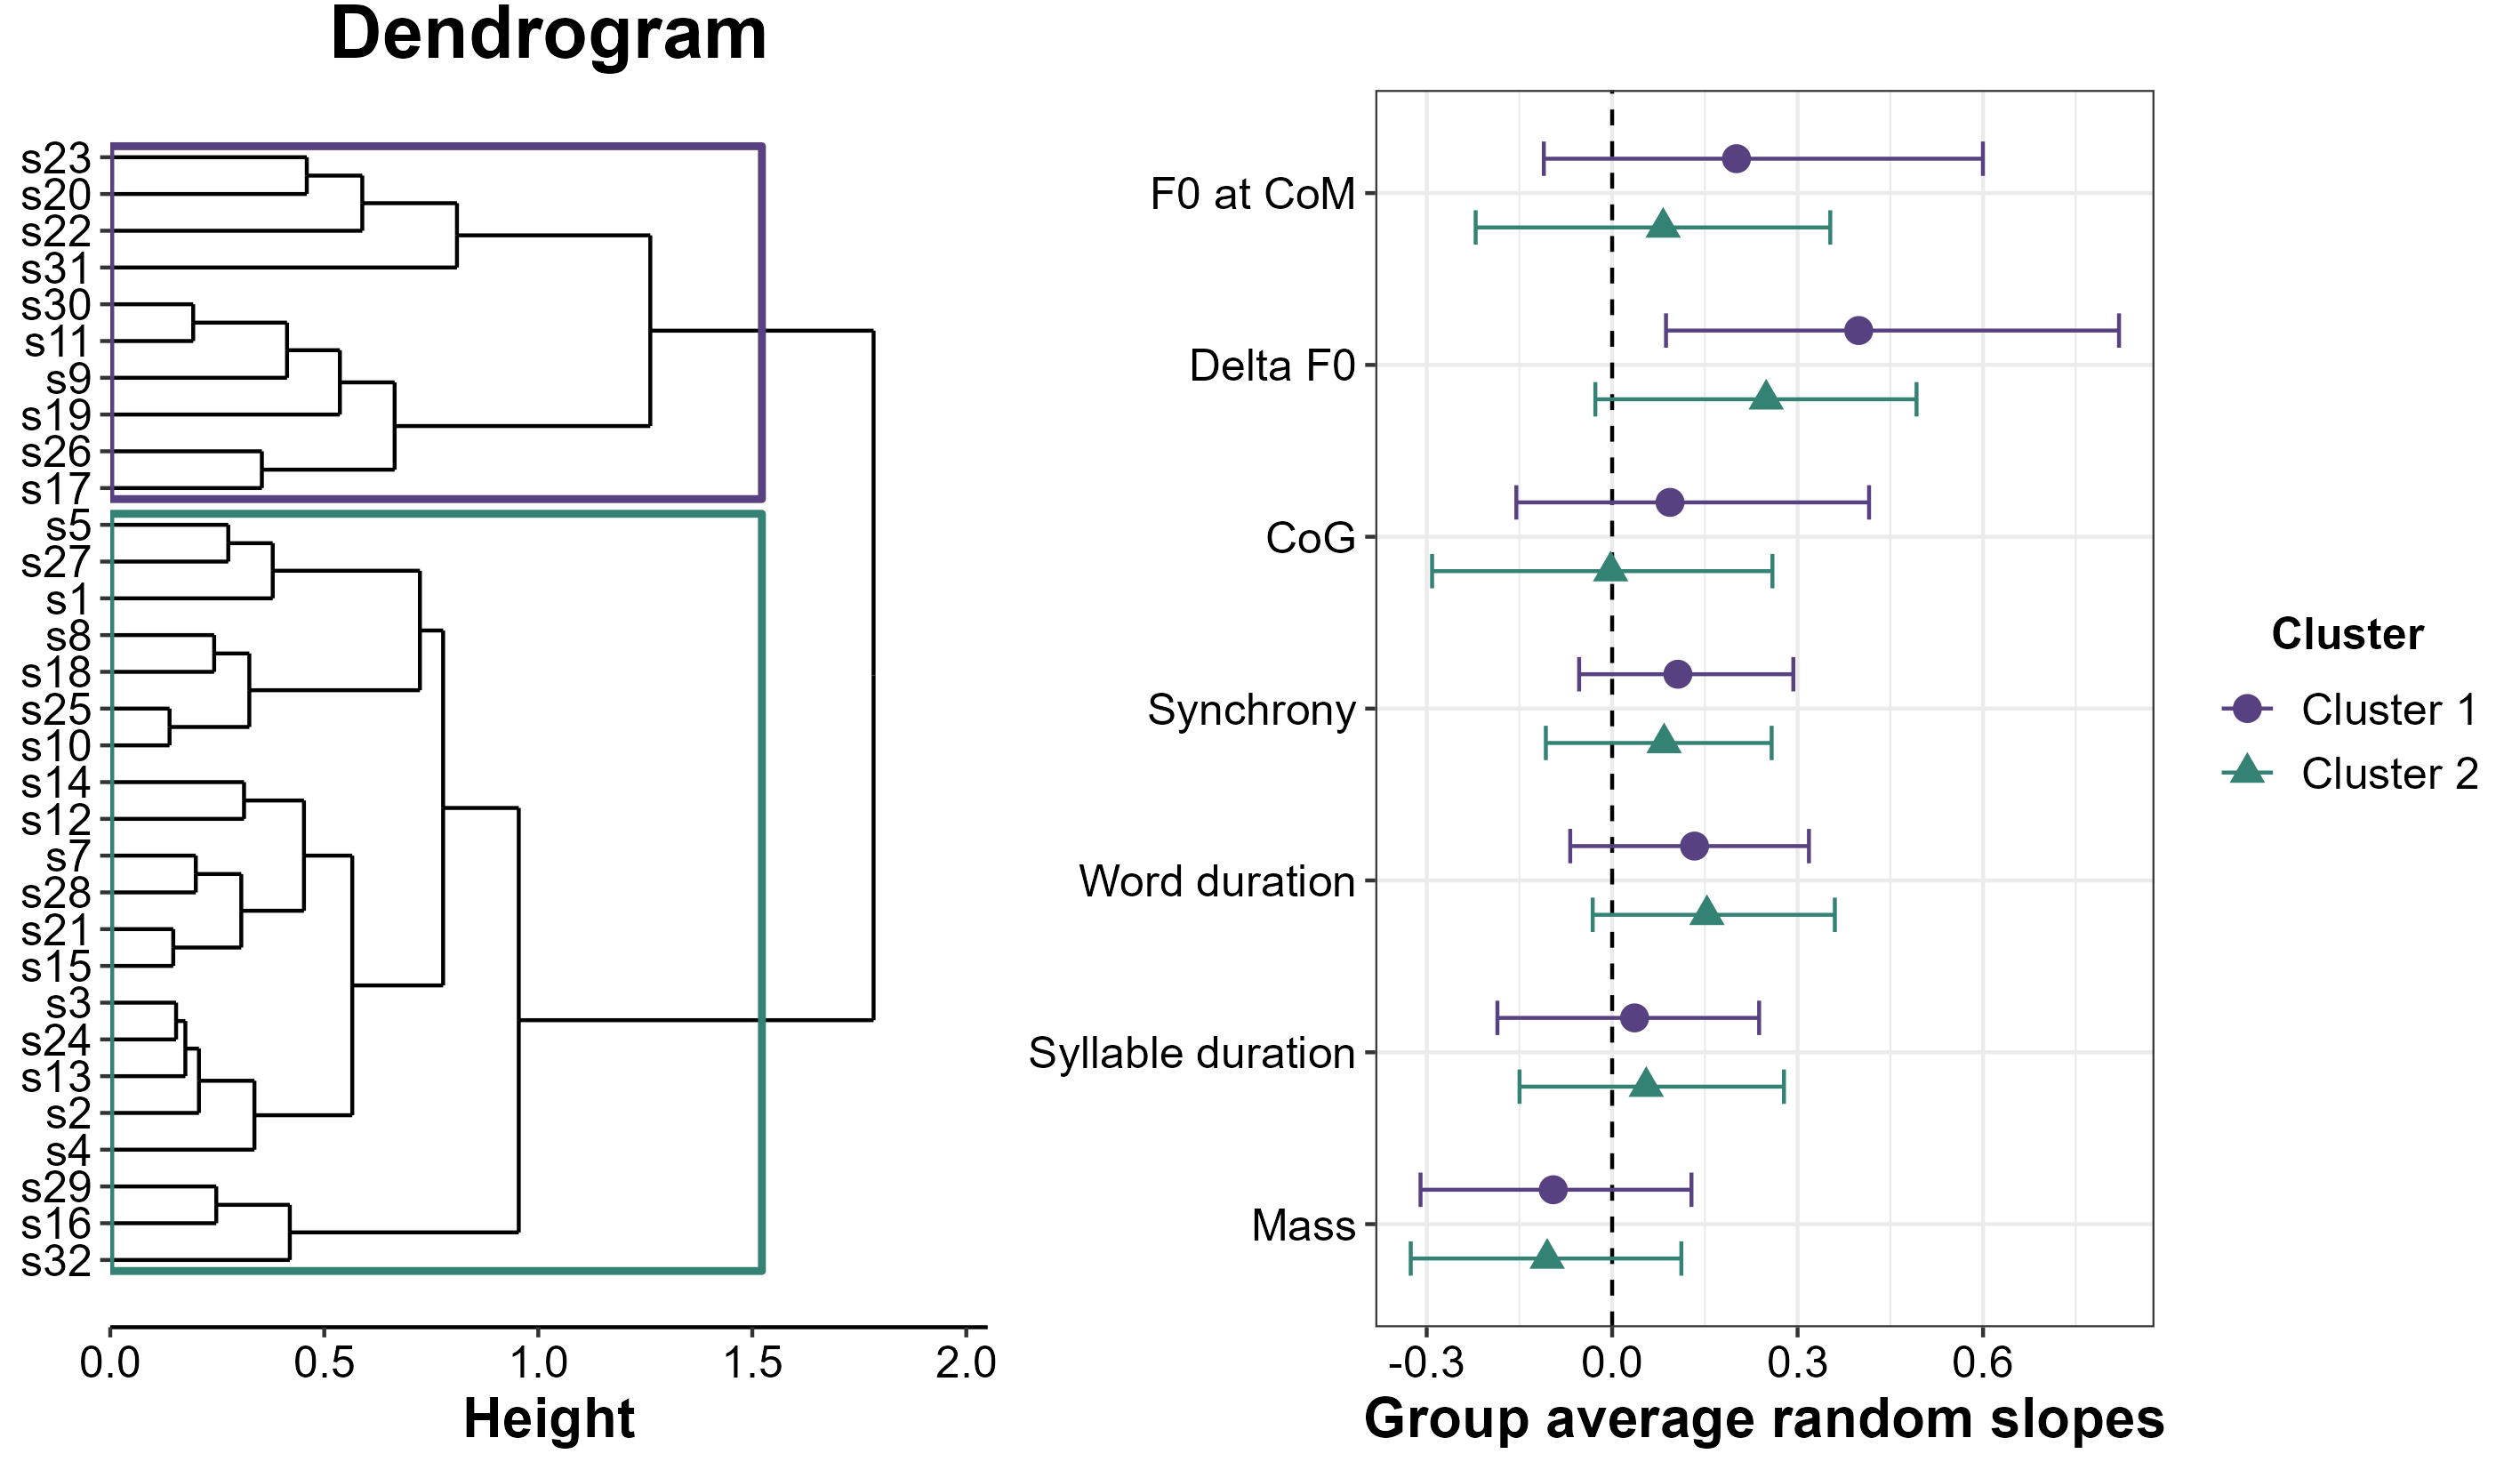
\includegraphics[width=\textwidth]{s1_clusters}
	\caption{Results of cluster analysis. Left: Dendrogram showing cluster affiliations of all speakers. Right: Plot showing the group averages and 90\% CrIs per cluster for each prosodic parameter.}
	\label{fig:s1_clusters}
\end{figure}

In order to illustrate what characterizes these clusters, Figure \ref{fig:s1_clusters} (right) shows the group averages and 90\% CrIs of the random slope coefficients for every parameter per cluster, thus visualizing the differences and similarities between the clusters. A positive value here indicates that a parameter has higher values in the new than in the accessible referents, i.e., that the parameter is used in the expected direction, marking new referents as more prominent than accessible ones. As evident from this plot, Cluster 1 appears to mark information status more strongly than Cluster 2 in terms of the four F0-related parameters F0 at CoM, Delta F0, CoG, and synchrony. Regarding word and syllable duration, the relation is reversed with Cluster 2 producing slightly larger differences between new and accessible than Cluster 1. However, it should be noted that especially for syllable duration, the differences between new and accessible referents are very small with a mean close to zero for both clusters. 

The cluster analysis gives an approximation as to what may be the main distinguishing factor between groups of speakers, namely, the strength of encoding of information status. Nevertheless, overall, the two clusters are remarkably similar, Delta F0 being the most important parameter for both groups of speakers. However, the cluster analysis coarsely groups speakers together and thus is not able to capture the full extent of individual variability that was observed in the descriptive analysis above. The implications of the choice of methodology for looking at individual variability will be further discussed in Section \ref{sec:Production 1 discussion} below.

To integrate observations of how speakers differ in their usage of continuous phonetic cues to information status on the one hand and categorical phonological cues on the other, Figure \ref{fig:s1_statustype_bycluster} plots the number of speakers in a cluster by whether they use accent status and accent type in the expected direction to encode information status, i.e., produce more nuclear and more prominent pitch accents in new than in accessible referents. Most of the speakers in Cluster 1 do not use accent status as a cue to information status. In Cluster 2, by contrast, there is a relatively even split into speakers who use accent status and speakers who do not. As a reminder, Cluster 1 includes the speakers that use the continuous phonetic measures (at least those related to F0) more strongly to encode information status than those in Cluster 2. Somewhat unexpectedly, the distribution of speakers who do or do not use accent status as a cue to information status suggests the reverse, namely, that Cluster 2 more strongly marks information status via prosodic structure. However, there was also a very subtle trend for speakers in Cluster 2 to use duration more effectively than those in Cluster 1. Cluster 2 could thus be regarded as a group of speakers that are more reliant on aspects related to timing, encompassing both accent status and duration, to mark information status.

By contrast, the results regarding accent type usage (see Figure \ref{fig:s1_statustype_bycluster}) seem to be in line with the strong versus weak encoders split observed with regard to the continuous prosodic parameters: All speakers in Cluster 1 (the strong phonetic encoders) use accent type in at least one position (Word1 or Word2) to mark information status, while in Cluster 2, seven speakers do not use accent type at all. What is more, half of the speakers in Cluster 1 use accent type as a cue in both positions, while only a quarter of speakers in Cluster 2 do the same. Accent type thus reflects the findings with regard to the continuous parameters emerging from the cluster analysis. Or, conversely, the continuous F0-related parameters are able to adequately capture aspects characterizing accent type categories. 

\begin{figure}
	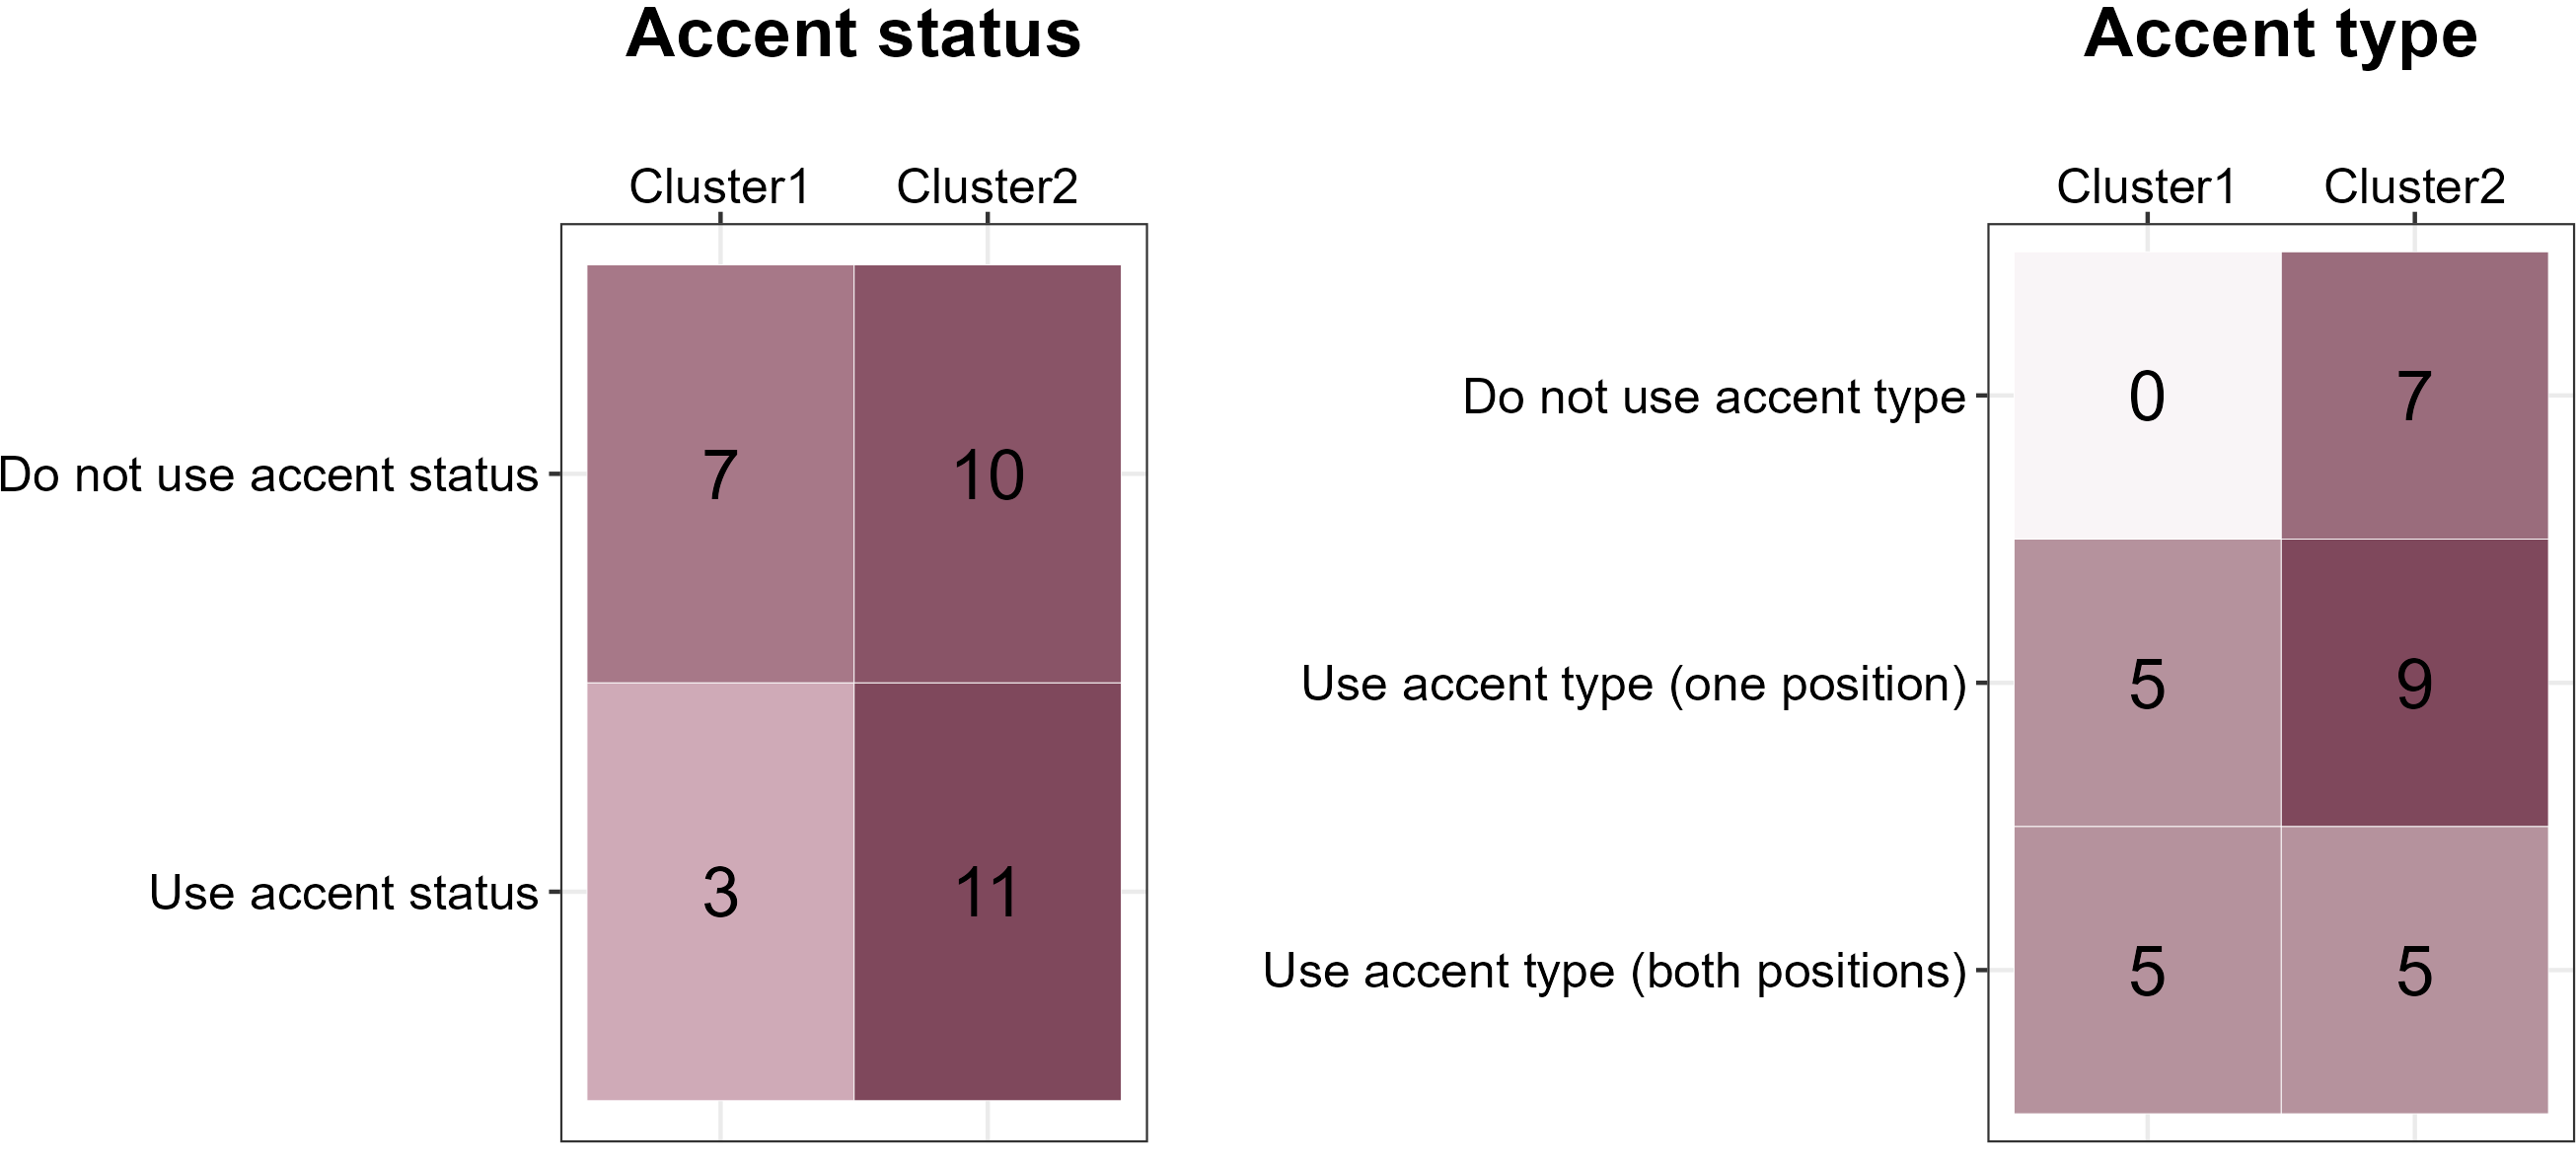
\includegraphics[width=\textwidth]{s1_accent_statustype_bycluster_cropped}
	\caption{Plot showing the number of speakers using accent status in Word1 (left) and accent type (right) to encode information status as a function of the cluster they belong in.}
	\label{fig:s1_statustype_bycluster}
\end{figure}

For completeness, a brief note on sociodemographic characteristics of the two clusters is in order. Since this is not the primary objective of the present study, we can only characterize the speakers in terms of their age, gender, and region of origin (see Table \ref{table:s1_sociodemographics}). Speakers associated with Cluster 1 are slightly older than those associated with Cluster 2, although the difference is only three years. The gender distribution is relatively balanced across clusters: 70\% of speakers in Cluster 1 are female compared to 76\% of speakers in Cluster 2. Finally, speakers in Cluster 1 are more likely to originate from the south of Germany (Bavaria, Baden-Wuerttemberg, and Thuringia) than speakers in Cluster 2, where 57\% of speakers are from the north (Lower Saxony, Schleswig-Holstein, Hamburg, and North Rhine-Westphalia). Generally, these observations reflect the relatively uniform age group from which participants were recruited and the skewed gender balance. In light of these shortcomings and the lack of clear tendencies, we will return to the examination of potential sociodemographic effects in the General Discussion (Chapter \ref{ch: general discussion}) after having added further data points in the following two studies.

\begin{table}[]
\begin{tabular}{lrr}
\lsptoprule
                 & Cluster 1 \newline n = 10    & Cluster 2 \newline n = 21    \\
                 \midrule
Age (median)     & 28                     & 25                     \\
Gender           & 70\% female, 30\% male & 76\% female, 24\% male \\
Region of origin & 30\% north, 70\% south & 57\% north, 43\% south \\
\lspbottomrule
\end{tabular}
\caption{Sociodemographic characteristics of the two clusters.}
\label{table:s1_sociodemographics}
\end{table}

\section{Interim discussion} \label{sec:Production 1 discussion}

Across speakers, Delta F0 emerged as the strongest correlate of information status in our data, new referents being produced on average with higher Delta F0 than accessible referents. In addition, new referents were reliably produced with more prominent accent types and there was a strong tendency for new referents (in Word1) to be realized with a nuclear as opposed to a prenuclear accent. There was also some evidence that F0 at CoM, synchrony, and word duration play a role in information status marking, which was, however, modulated by position in the sentence: New referents in Word1 were produced with on average higher F0 at CoM than accessible referents, new referents were on average longer than accessible ones, more so in Word1 than in Word2, and had higher synchrony values, particularly in Word2. CoG, syllable duration, and periodic energy mass were of little to no importance in the encoding of information status. The overall results on the group level are generally reflected on the individual level, with Delta F0 being the cue used by most speakers (25 out of 32). This finding underlines the predominance of F0 as a correlate of prominence \citep[e.g.,][]{bolingerTheoryPitchAccent1958, fryExperimentsPerceptionStress1958, liebermanAcousticCorrelatesWord1960, baumannWhatMakesWord2018, roessigTracingPhoneticSpace2022} not only in averaged data but also for the individual speaker.

As per the cluster analysis performed on the models' random slopes, speakers were very similar in their encoding of information status, particularly in the direction of effects observed for all seven prosodic parameters. Nevertheless, the cluster analysis revealed a split into two groups, each employing a slightly distinct strategy. The main difference between these two strategies lies in the extent to which speakers modulated any given parameter, i.e., the strength of encoding: Cluster 1 (consisting of fewer speakers) marked a larger difference between new and accessible target words than Cluster 2 (the larger cluster of the two). These results are in line with previous findings that some speakers encode certain pragmatic contrasts more effectively than others \citep[e.g.,][]{cangemiListenerSpecificPerceptionSpeakerSpecific2015}. Such speakers are either better communicators who consciously (or unconsciously) mark pragmatic contrasts (such as newness) more clearly in order to facilitate interpretation of utterances on the side of the listener or they are more sensitive to such pragmatic contrasts which enables them to mark them prosodically.

Especially in perception studies, higher sensitivity to pragmatic contrasts encoded via prosody has been linked to concepts such as pragmatic/communicative skill or empathy \citep{bishopPhonologyPhoneticsSignalextrinsic2020, orricoInfluenceEmpathyAutisticlike2023}. Analogously, in production, speakers with higher pragmatic skill or empathy would be expected to encode pragmatic contrasts more strongly than speakers with lower pragmatic skill, which could explain the difference in strength of encoding observed in our data. However, recent production studies investigating the relation between pragmatic skill and contrastiveness of categories find only subtle if not inconclusive effects \citep{turnbullListenerorientedPhoneticReduction2019, bishopBriefReportAutistic2022}.

Beyond the difference in the strength of encoding of information status, we found more diverse strategies on the individual level in the choice of parameters used to encode information status when considering the raw data. One potential reason enabling this variability is the acoustic redundancy that is present in the signal. In West Germanic languages, prosodic prominence is encoded via the F0 contour, duration, and intensity and it is assumed that all three acoustic dimensions play a role in the prosodic marking of pragmatic contrasts, such as information status. Functional redundancy in speech ensures the robustness of the message and guarantees communicative success in noisy situations \citep{winterSpokenLanguageAchieves2014}. This opens up the possibility for individual speakers to make use of only some of the available prosodic parameters without losing the ability to successfully encode the intended meaning. In our data, there are speakers who rely solely on F0-related cues, while others use only changes in duration to encode information status, thus efficiently exploiting the functional redundancy in the signal. In fact, speakers rarely make use of the full range of cues available to them. Out of our 32 speakers, only one encodes information status maximally redundantly. Similar ``cue-trading" effects have also been observed in \citet{severijnenYourVOORnaamNot2024} in the encoding of word-level stress in Dutch, where speakers who used higher mean F0 to mark stress were less likely to rely on intensity.

Integrating the continuous and categorical results at the individual level revealed a surprising asymmetry: While the strong phonetic encoders were also more likely to use accent type as a cue to information status than the weaker encoders, the relation was reversed for accent status. Weaker phonetic encoders, who showed a slightly stronger preference for using duration, were more likely to use accent status than stronger phonetic encoders (but note again that accent status can only be used as a cue in Word1, since Word2 is always produced with a nuclear accent). Speakers may split into those who modify timing (including accent status) and those that modify the shape of the F0 contour, which is reflected in both accent type choice and the phonetic parameters measuring F0. Interestingly, this split reflects the dichotomy between metrical structure (or relative prominence) and tune (or pitch) that lies at the heart of influential theories of intonational phonology (e.g., \citealt{laddIntonationalPhonology2008}, see also Section \ref{section: structural prominence}). Metrical structure describes the alternation of strong and weak entities at the sentence level, while tune refers to the alternation of rises and falls in the F0 contour. These two aspects are orthogonal to each other and are independently variable \citep{laddIntonationalPhonology2008}. In the present data, accent status and duration are manifestations of metrical structure that are used to encode information status by the same group of speakers, while accent type and the continuous F0 measures capture variability in the tune. The results may suggest that not only are tune and metrical structure independently manipulable, but that individual speakers may have preferences regarding which of the two aspects they modify to encode a semantic-pragmatic contrast, such as information status. This hypothesis will be further discussed in Chapter \ref{ch: general discussion}. 

Arguably, a change in metrical structure should be more consequential for the listener than F0 modulations, as it has been shown in previous studies that accent status is among the most important cues to the perception of prominence \citep{baumannWhatMakesWord2018}. Thus, when it comes to perception, the group of speakers modifying accent status might emerge as the overall stronger encoders than the group that use accent type and F0-related parameters to a larger extent to encode information status. However, our study lacks variability in the likely most important categorical prosodic cue to prominence, i.e., the presence or absence of a pitch accent \citep[e.g.,][]{baumannWhatMakesWord2018, wagnerExploitingSpeechgestureLink2019}, since all of our target words were accented. Speakers that use accent status as a cue to the accessible-new contrast could also be more likely to vary accentuation patterns in marking other pragmatic contrasts (e.g., a given-new contrast), which would make them more successful in communicative settings than the accent type and F0 encoders. This is a matter for further investigation.

In the present study, we investigated individual variability via two different approaches: Descriptively, by examining the distributions of the prosodic parameters for each speaker and by performing a cluster analysis on the random slope coefficients of mixed-effects models. These approaches differ substantially and emphasize different aspects in the study of inter-speaker variability. While the cluster analysis aims to identify common strategies shared by multiple speakers in an objective manner, the descriptive method allows for an in-depth exploration of every single speaker. Crucially, the cluster analysis method is fairly conservative in estimating differences across speakers, instead emphasizing similarities. This is a consequence of using random slope coefficients as input for the clustering. Random slopes account for by-speaker variation in the effect of a predictor \citep[e.g.,][]{winterStatisticsLinguistsIntroduction2020}, in our case information status. However, random slopes are not estimated independently for each individual but always together with and in relation to the group-level estimates. This means that the by-speaker estimates are drawn towards the overall mean effect, a process known as ``shrinkage" \citep[271-272]{winterStatisticsLinguistsIntroduction2020}. Nevertheless, the cluster analysis provides valuable insight into different strategies employed by groups of speakers in a manageable, straightforward-to-interpret way. The descriptive exploration, by contrast, reveals that there are more diverse strategies in the data than the cluster analysis suggests. However, this may over-emphasize individual variability, especially in the light of relatively few data points per speaker, which is arguably the case in our data set. Running the cluster analysis on the ``shrunken" random slope estimates thus gives the results more statistical validity. Much can therefore be gained by considering insights from both approaches.

The present chapter has provided an exploratory account of individual differences and similarities in the prosodic marking of information status. However, several questions remain unanswered. As has already been shown by \citet{cangemiListenerSpecificPerceptionSpeakerSpecific2015}, more redundant prosodic encoding of pragmatic contrasts facilitates their interpretation on the side of the listener. However, it remains unclear how the listener deals with contradictory cues. For example, there are cases in our data where a speaker produces new words on average with longer duration than accessible ones, yet accessible words exhibit more extensive F0 rises (or vice versa).

Furthermore, this study describes the nature of inter-speaker variability but provides no potential causes of them. In a further study, we will consider communicative skill as a potential predictor of individual differences, which has previously yielded promising results, particularly in perception studies \citep{bishopPhonologyPhoneticsSignalextrinsic2020, orricoInfluenceEmpathyAutisticlike2023}. Finally, the present study considered only information status as a factor to be encoded via prosodic prominence. We will expand on this by taking into account other (semantic-pragmatic and syntactic) factors to see whether comparable patterns of across-speaker differences and similarities emerge in their encoding via prosodic prominence. Chapter \ref{ch:Production II} aims to address some of these issues.
